%%%%%%%%%%%%%%%%%%%%%%%%%%%%%%%%%%%%%%%%%%%%%%%%%%%%%%%%%%%%%%%%%%%%%%%%%%%%%%%%%%%%%%%%%%%%%%%%%%%%%%%%%%%%%%%%%%%%%%%%%%%%%%%%%%%%%%%%%%%%%%%%%%%%%%%%%%%
% This is just an example/guide for you to refer to when submitting manuscripts to Frontiers, it is not mandatory to use Frontiers .cls files nor frontiers.tex  %
% This will only generate the Manuscript, the final article will be typeset by Frontiers after acceptance.   
%                                              %
%                                                                                                                                                         %
% When submitting your files, remember to upload this *tex file, the pdf generated with it, the *bib file (if bibliography is not within the *tex) and all the figures.
%%%%%%%%%%%%%%%%%%%%%%%%%%%%%%%%%%%%%%%%%%%%%%%%%%%%%%%%%%%%%%%%%%%%%%%%%%%%%%%%%%%%%%%%%%%%%%%%%%%%%%%%%%%%%%%%%%%%%%%%%%%%%%%%%%%%%%%%%%%%%%%%%%%%%%%%%%%

%%% Version 3.4 Generated 2018/06/15 %%%
%%% You will need to have the following packages installed: datetime, fmtcount, etoolbox, fcprefix, which are normally inlcuded in WinEdt. %%%
%%% In http://www.ctan.org/ you can find the packages and how to install them, if necessary. %%%
%%%  NB logo1.jpg is required in the path in order to correctly compile front page header %%%

\documentclass[utf8]{FrontiersinHarvard} % for articles in journals using the Harvard Referencing Style (Author-Date), for Frontiers Reference Styles by Journal: https://zendesk.frontiersin.org/hc/en-us/articles/360017860337-Frontiers-Reference-Styles-by-Journal

\usepackage{url,hyperref,lineno,microtype}
\usepackage{xr}
\usepackage{amssymb}
\usepackage{amsmath, bm}
\usepackage{mathabx}
\usepackage{siunitx}
\let\DeclareUSUnit\DeclareSIUnit
\let\US\SI
\DeclareUSUnit\inch{in}
\DeclareUSUnit\ft{ft}
\providecommand{\abs}[1]{\lvert#1\rvert}
\providecommand{\norm}[1]{\lVert#1\rVert}
\usepackage{graphicx}
\graphicspath{{../}} % figures live in Knee_Torque_Test/Figures (Ben's structure); on Overleaf Figures/ sits beside Main.tex
\usepackage{caption}
\usepackage{tabularx}
\usepackage{booktabs}
\usepackage{multirow}
\usepackage{float}
\usepackage{array}
\usepackage[onehalfspacing]{setspace}
\renewcommand{\arraystretch}{2}  % Increase row height (default is 1.0)
\linenumbers

\externaldocument{frontiers_SupplementaryMaterial}

% Leave a blank line between paragraphs instead of using \\
\def\keyFont{\fontsize{8}{11}\helveticabold }

\def\firstAuthorLast{Bolen {et~al.}} %use et al only if is more than 1 author

\def\Authors{Ben Bolen\,$^{1,*}$, Lindie Burgess\,$^{1}$, Connor Morrow\,$^{1}$, and Alex Hunt\,$^{1}$}
% Affiliations should be keyed to the author's name with superscript numbers and be listed as follows: Laboratory, Institute, Department, Organization, City, State abbreviation (USA, Canada, Australia), and Country (without detailed address information such as city zip codes or street names).
% If one of the authors has a change of address, list the new address below the correspondence details using a superscript symbol and use the same symbol to indicate the author in the author list.

\def\Address{$^{1}$Agile and Adaptive Robotics Laboratory, Portland State University, Department of Mechanical and Materials Engineering, Portland, OR, USA }
% The Corresponding Author should be marked with an asterisk
% Provide the exact contact address (this time including street name and city zip code) and email of the corresponding author
%\def\corrAuthor{Ben Bolen, Portland State University, Department of Mechanical and Materials Engineering, 1930 SW 4th Ave., Portland, OR, 97207, USA}

\def\corrAuthor{Ben Bolen \\ Portland State University \\ Department of Mechanical and Materials Engineering \\ PO Box 751 \\ Portland, OR, 97207-0751, USA}


\def\corrEmail{bbolen83@gmail.com}

\begin{document}

\onecolumn

\firstpage{1}

\title[Design Factors for Isometric Robotic Knee Torque]{Design Factors for Isometric Robotic Knee Torque Using Braided Pneumatic Actuators} 

\author[\firstAuthorLast ]{\Authors} %This field will be automatically populated
\address{} %This field will be automatically populated
\correspondance{} %This field will be automatically populated
\extraAuth{}% If there are more than 1 corresponding author, comment this line and uncomment the next one.
%\extraAuth{corresponding Author2 \\ Laboratory X2, Institute X2, Department X2, Organization X2, Street X2, City X2 , State XX2 (only USA, Canada and Australia), Zip Code2, X2 Country X2, email2@uni2.edu}
\maketitle%
\begin{abstract}

%%% Leave the Abstract empty if your article does not require one, please see the Summary Table for full details.
\section{}
Artificial muscles such as braided pneumatic actuators (BPAs) reproduce the force and contraction behavior of skeletal muscle, making them attractive for the legs of musculoskeletal robots. However, the isometric torque a BPA delivers about a joint remains difficult to predict, because rigid-body torque models omit attachment compliance, effective-length offsets, and the contraction lost where the actuator wraps over the joint. In this work, we measured isometric knee torque on pinned and biomimetic knee test stands across actuator resting lengths, isolated error sources with a hybrid torque calculation, and identified correction terms by multiobjective optimization. Our analysis resulted in (1) a corrected torque model whose length offset, effective stiffness, and fictive-strain wrapping loss, expressed through the unloaded \qty{620}{\kPa} contraction, cut held-out prediction error by two thirds or more on the pinned-knee test families and transfer to the biomimetic knee without refitting; (2) a cross-configuration-consistent stiffness pair selected by a simultaneous design requirement; and (3) redesigned attachment routes that meet or exceed human isometric knee-torque targets with quantified margins, together with the first hardware torque measurements of the redesigned extensor route. The corrected model and redesign pipeline support first-iteration torque design of BPA-actuated robot joints.

\tiny
 \keyFont{ \section{Keywords:}
Braided Pneumatic Actuator, Artificial Muscle, Isometric Torque, Moment Arm, System Identification, Actuator Routing, Biomimetic Robotics, Knee Joint}
 %All article types: you may provide up to 8 keywords; at least 5 are mandatory.
\end{abstract}

\section{Introduction}

Musculoskeletal robots built on biological design principles are experimental platforms for motor-control questions that are impractical or unethical to study in human subjects, from spinal reflex loops to the coupling of posture and locomotion \citep{ijspeert_amphibious_2020, goldsmith_investigating_2021, liu_robotic_2018}. The same principles also yield machines that copy the anatomy of their biological counterparts: human-mimetic humanoids and anthropomorphic arms with anatomically arranged musculotendon networks \citep{asano_design_2017, asano_musculoskeletal_2019, hitzmann_anthropomorphic_2018}, lower-limb robots driven by multifilament muscles \citep{kurumaya_musculoskeletal_2016}, and platforms that isolate the function of a single muscle such as the gluteus medius \citep{shin_constructive_2018} or select actions during adaptive locomotion \citep{schilling_adaptive_2022}. Each of these machines asks its actuators to do what skeletal muscle does: pull as a lightweight tension member whose force depends on excitation and length, routed from origin to insertion across a joint. The joint-level quantity that matters is not force but torque, and torque depends as much on the routed path as on the actuator itself.

No actuator family reproduces muscle exactly, and each alternative trades something away. Geared electric motors dominate position control, but they place mass and reflected inertia at the joint and gain compliance only through added series elasticity \citep{veale_towards_2016}. Hydraulics supply high force density at the price of pumps, valves, and rigid supply lines \citep{suzumori_trends_2018}. Shape-memory alloys respond slowly, and dielectric elastomers deliver low force at impractical drive voltages \citep{madden_artificial_2004}. Braided pneumatic actuators (BPAs), also called McKibben artificial muscles, occupy the practical middle ground: a pressurized sleeved bladder that shortens and pulls, producing force that falls with contraction in a muscle-like way while remaining a compliant tension member. Air-muscle quadrupeds have demonstrated robust, adaptive gaits \citep{aschenbeck_design_2006}, and the Festo fluidic BPAs used in this work are commercially available in the sizes a human-scale leg requires.

For BPAs, the force side of the design problem is well characterized: we have published closed-form equations for the maximum force and the isometric force of \qtylist{10;20}{\mm} Festo actuators as functions of pressure, contraction, and resting length \citep{bolen_2026}. The torque side has received far less attention. Joint torque is the product of actuator force and the moment arm of the actuator's line of action about the joint axis, and the moment arm is a property of the attachment route that changes with joint angle. Biomechanics treats moment-arm determination as its own measurement problem, from lower-limb muscular anatomy \citep{brand_model_1982} and three-dimensional musculotendon estimation \citep{menegaldo_moment_2004} to curved paths with moving attachment points \citep{suderman_moving_2012}, because short moment arms amplify path error \citep{young_analyzing_2019}. A robot designer adds effects that no biological model carries: brackets and fixtures deform under load, artificial tendons and cabling stretch, and at deep flexion the actuator bends over the joint and loses usable contraction. None of these effects appears in a rigid-body torque model built from a characterized actuator and nominal geometry.

Torque modeling for braided actuators has consequently concentrated on the force law and on placement. \citet{chou_measurement_1996} derived the static force relation of McKibben muscles from braid geometry and quantified its hysteresis, and later work refined static models and approximations for pneumatic and fluidic muscles \citep{tondu_static_2022, sarosi_new_2012}. For the actuator family used here, \citet{martens_modeling_2017} modeled static force from a geometric and material framework, and \citet{hunt_modeling_2017} modeled length effects. At the joint level, \citet{bolen_determination_2019} determined artificial-muscle placement for biomimetic humanoid robot legs, and \citet{morrow_optimization_2020} optimized placements so that a bipedal robot matches human torque and range-of-motion capabilities. What these models do not provide is a torque prediction that survives contact with a physical joint. None of them represents fixture and tendon compliance in the load path, carries an effective-length offset between modeled and physical muscle length, or accounts for the contraction lost where the actuator wraps over the joint. To our knowledge, no BPA torque model has been validated across joint configurations, actuator resting lengths, and both antagonistic sides of a joint with a single consistent parameter set.

The present work treats these mispredictions as identifiable design factors, not residual noise. We measured isometric knee torque on two test stands: a robot leg with a pinned revolute knee, and the same leg with a biomimetic knee whose instantaneous center of rotation migrates with flexion like that of the human joint \citep{steele_biomimetic_2018, steele_development_2017}. Each knee was driven by antagonistic flexor and extensor BPAs of \qtylist{10;20}{\mm} diameter across a range of resting lengths, with and without artificial tendons. A hybrid torque calculation, which combines measured muscle lengths and moment arms with modeled actuator force, isolated kinematic error from force error before any parameter was fitted.

Our analysis resulted in (1) a corrected torque model whose constant length offset ($\chi_0$), lumped attachment stiffness ($\chi_1$ and $\chi_2$), and fictive-strain wrapping loss ($\chi_3$) cut held-out prediction error by two thirds or more on the pinned-knee test families and carry to the biomimetic knee without refitting; (2) a two-stage multiobjective identification that holds one stiffness pair consistent across both knees and both actuators, validates it on held-out resting lengths and on the biomimetic knee, and selects the adopted set by an external design requirement; and (3) redesigned attachment routes, each driven by two \qty{20}{\mm} BPAs, that meet or exceed human isometric knee-torque targets from OpenSim musculoskeletal models \citep{seth_opensim_2018, delp_interactive_1990} with a required \qty{5}{\percent} margin at every angle, together with the first hardware torque measurements of the redesigned extensor route. Throughout, the wrapping loss is expressed through fictive strain: the excess contraction the force model must see beyond the actuator's physical contraction, normalized by the unloaded \qty{620}{\kPa} contraction $\varepsilon_{620}$ of the free actuator. Together, the corrected model and the redesign pipeline let a designer predict isometric joint torque, correct it against hardware, and route the actuators to a human-derived target on the first design iteration.


\section{Methods and Materials}\label{sec:methods}

\subsection{Overview}

Isometric knee torque is the product of the force an actuator develops and the moment arm of its line of action about the joint axis, and the force itself is set by the actuator's effective length through the force model. Each link in that chain is a design quantity: the attachment routing fixes the moment arm, the resting length and attachment compliance set the effective contraction, and wrapping over the joint removes usable length. We built two knee test stands, measured isometric torque across each joint's range of motion with \qtylist{10;20}{\mm} Festo braided pneumatic actuators (BPAs) in flexor and extensor configurations, and compared the measurements against the original rigid-body model, the improved actuator force characterization alone, and the corrected model developed here. A hybrid calculation isolated the error sources, a multiobjective identification produced the correction terms, and the corrected model then drove a redesign of the attachment routes against human isometric torque targets.

\subsection{Actuator Force Model}\label{sec:force_model}

The actuator force model is fully described in \citet{bolen_2026} and is reproduced here only as far as the torque model requires. The contraction $\varepsilon$ of a BPA is
\begin{equation}
    {\varepsilon} = \frac{(l_{0}-l_\text{m})}{l_{0}} \label{eq:strain}
\end{equation}
where $l_{0}$ is the uninflated resting length measured from hose clamp to hose clamp and $l_\text{m}$ is the current muscle length. The unloaded contraction at \qty{620}{\kPa} is
\begin{equation}
    \varepsilon_{620} = \frac{(l_{0}-l_{620})}{l_{0}} \label{eq:max_strain}
\end{equation}
where $l_{620}$ is the actuator length at \qty{620}{\kPa} with no external load, and the relative contraction is
\begin{equation}
    \varepsilon^* = \frac{\varepsilon}{\varepsilon_{620}} \label{eq:rel_strain}
\end{equation}
The pair $(\varepsilon_{620}, \varepsilon^*)$ is the strain basis of this work: every length-based correction introduced below is expressed in $\varepsilon_{620}$-normalized units. The normalized isometric force is
\begin{equation}
F^*(\varepsilon^*,P^*)=
\begin{cases}
\begin{aligned}
c_0\cdot\bigl(\exp(-c_1 \cdot \varepsilon^*)-1\bigr)
+ P^*\cdot\exp\!\bigl(-c_2(\varepsilon^*)^{2}\bigr)
\end{aligned}
& \text{where positive}\\[10pt]
0
& \text{otherwise,}
\end{cases}\label{eq:Fstar}
\end{equation}
that is, the normalized force is the value of the bracketed expression where that expression is positive and zero elsewhere, where $P^*$ is pressure normalized by \qty{620}{\kPa} and the diameter-dependent coefficients $c_0$, $c_1$, and $c_2$ are tabulated in \citet{bolen_2026} (p.~10). The maximum force is
\begin{equation}
    F_{\mathrm{max}}(l_{0},P) = a_1 \, P \, \arctan\!\bigl(a_2 \, P \, (l_{0}-0.0075)\bigr) \label{eq:Fmax_3D}
\end{equation}
with $l_{0}$ in meters, a fixed \qty{7.5}{\mm} end-contact offset, and coefficients tabulated in \citet{bolen_2026} (p.~7); at the \qty{620}{\kPa} system ceiling, $F_{\mathrm{max}}(l_{0},\qty{620}{\kPa}) = F_{620}(l_{0})$. The isometric force is the composition
\begin{equation}
   F(\varepsilon^*,P^*,l_{0}) = F^*(\varepsilon^*,P^*) \cdot F_{620}(l_{0}) \label{eq:force}
\end{equation}

\subsection{Robot Leg Model and Knee Test Stands}\label{sec:robot_model}

The robot leg consists of a knee joint, femur, tibia, BPA assemblies, and artificial tendons (Figure~\ref{fig:testJigs}\textbf{A--C}). The artificial bones were 3D printed in Onyx, carbon fiber, and high-strength high-temperature fiberglass, with machined links for the knee mechanism, and the tendons are Shimano bicycle brake cable. The leg geometry and dimensions derive from bone scans of a \qty{6}{\ft} (\qty{1.83}{\metre}) tall person \citep{bolen_determination_2019,seth_opensim_2018,delp_interactive_1990,delp_opensim_2007}.

\begin{figure}[H]
    \begin{center}
    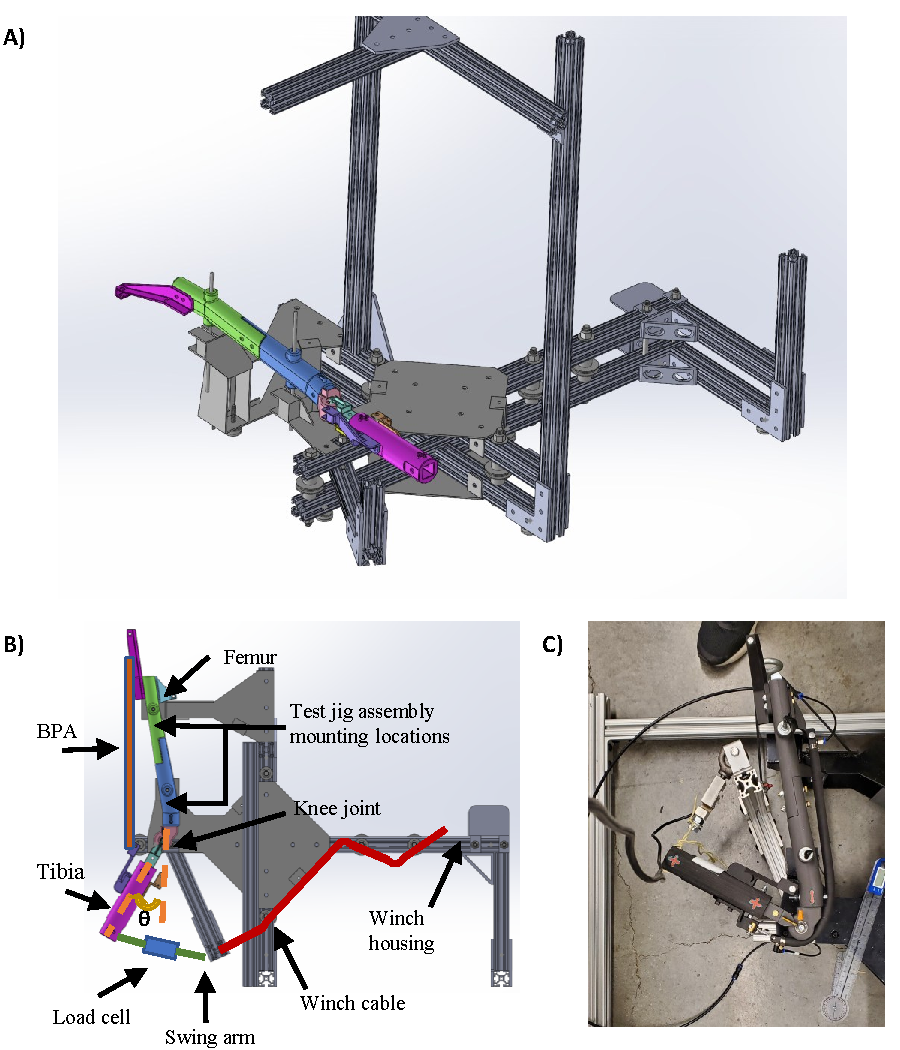
\includegraphics[width=0.9\textwidth]{Figures/testJigs.pdf}
    \end{center}
    \caption{\textbf{(A)} CAD solid model assembly of the revolute joint knee in the test stand. \textbf{(B)} 1-DoF pinned-joint robot knee in the test apparatus with important components labeled; the leg is shown with 30 degrees of flexion, i.e.\ $\theta_\text{k} = \ang{-30}$. \textbf{(C)} Picture from isometric torque testing. The setup shows the revolute knee configured for a test of the extensor BPA, with the knee flexed at $\theta_\text{k} = \ang{-120}$; note the compressed shape of the inflated BPA on the knee at this high degree of flexion.}\label{fig:testJigs}
\end{figure}

Two knee joints were tested: a pure revolute joint, and a biomimetic joint whose four-bar linkage translates the instantaneous center of rotation (ICR) as the knee rotates \citep{steele_biomimetic_2018,steele_development_2017,steele_biomimetic_2018-1}, moving it posteriorly in $X$ and distally in $Y$ in the femur frame, except briefly proximally near full flexion, much as the human knee does \citep{bolen_determination_2019}. Reference coordinate frames follow \citet{wu_for_1995,wu_isb_2002}, and Figure~\ref{fig:ICR} shows the measured ICR migration. Both joints share the same rotation center in the femur frame at $\theta_\text{k} = \ang{0}$, each was driven by an antagonistic flexor and extensor, and $\theta_\text{k}$ is negative in flexion throughout this work.

\begin{figure}[H]
    \begin{center}
    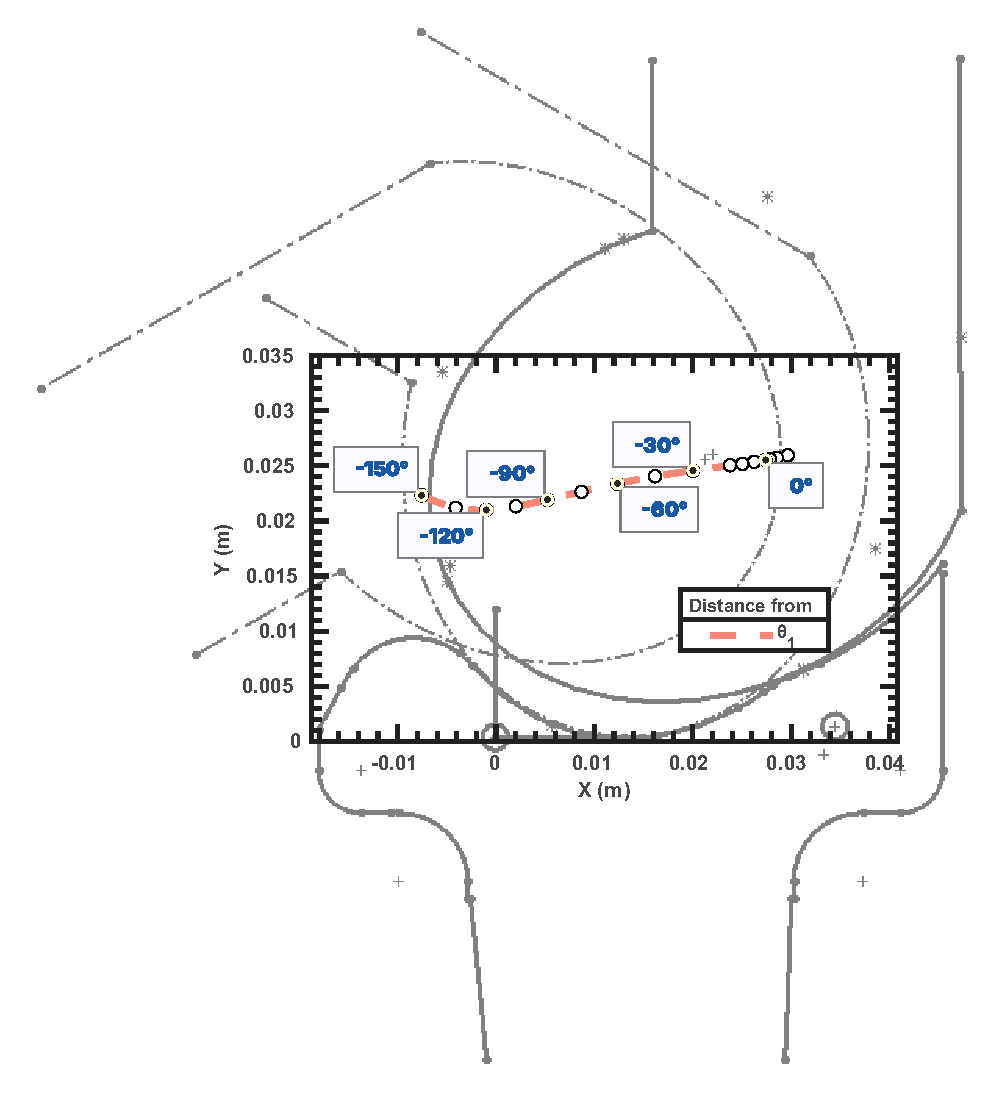
\includegraphics[width=0.8\textwidth]{Figures/KneeICR.eps}
    \end{center}
    \caption{ICR for the biomimetic robot knee as a function of knee angle, measured from $\theta_{1}$ on the tibia. The plot is overlaid on a model of the knee at $\theta_\text{k}=0^\circ$ (solid line) and $-60^\circ$ and $-120^\circ$ (dotted dash lines). White circles represent measured points in $-15^\circ$ increments from $-150^\circ$ to $-15^\circ$, in $-5^\circ$ increments from $-15^\circ$ to $0^\circ$, and then at $2^\circ$, $5^\circ$, and $10^\circ$.}\label{fig:ICR}
\end{figure}

Each stand was tested with $\diameter$\qty{10}{\mm} Festo BPAs in both configurations, and the biomimetic knee also with a $\diameter$\qty{20}{\mm} BPA. Each actuator was pinned at its origin on the femur, with the far end either pinned at the tibial insertion or attached there through an artificial tendon. \citet{bolen_determination_2019,morrow_optimization_2020} give full details of the modeled robot and its torque calculation.

\subsection{Equipment and Data Collection}\label{sec:torque_equipment}

A test jig was built to collect knee torque at set knee angles over the range of motion. The stand frame is made of 80/20 1515 series extruded aluminum. The femur is fixed to the frame while the knee rotates the tibia, with the joint axis co-axial with gravity to eliminate gravitational torque. A force sensor connects the tibia to a swing arm tied to a winch with 3/16-inch Kevlar rope (Quality Nylon Rope) routed over idler pulleys. At each measured $\theta_\text{k}$ the winch was locked and the BPA was inflated and then deflated, keeping the measurement as isometric as possible. Because the sensor and its rope load path tie the tibia to the locked winch, the sensor reading is the tension that holds the tibia at the set angle. The measured knee torque at each angle is that tension multiplied by the perpendicular distance from the knee axis to the rope's line of action at its tibial attachment, the measured counterpart of the scalar reduction of Equation~\eqref{eq:M_scalar}, with the attachment geometry and the sensor-line angle recorded at each test position.

Force was collected with one of two sensors: a MODERN STEP \qty{300}{\kilo\gram} digital crane scale, or a CALT DYLY-103 \qty{100}{\kilo\gram} S-shaped load cell used with an HX711 load-cell amplifier. Pressure was measured with a Freescale MPX5700 GP \qty{5}{\volt} pressure sensor. Supply pressure was controlled by two regulators in series, a Parker 20R113GC (\qtyrange{0}{120}{\psi}) and a Husky HDA72200, and air was delivered through a Festo VTUG-10 valve manifold. Pressure and load-cell data were sent to MATLAB through a Sparkfun BlackBoard C (Arduino Uno style) microcontroller. Lengths were measured with a tape measure, with a flexible string marking the axial length of the BPA when its curvature was sufficient, and angles with a Medigauge digital goniometer or MALENOO analog goniometers of \qtylist{6;8;12}{\inch} lengths.

\subsection{Hybrid Torque Calculation}\label{sec:hybrid_method}

Torque about the knee is the moment of the actuator force about the ICR. Two vectors enter it: the position vector $\mathbf{d}$ from the ICR to the point of force application, and the force vector $\mathbf{F} = \norm{\mathbf{F}}\hat{\mathbf{u}}$ along the line of action. The moment arm is the perpendicular distance from the joint axis to the line of action,
\begin{equation}
    r = \norm{\mathbf{d} \times \hat{\mathbf{u}}}
    \label{eq:momentarm_def}
\end{equation}
the same quantity computed from the vectors or measured with a tape measure. In the model it follows the projection method of \citet{young_analyzing_2019}: the scalar moment arm about the joint axis $\hat{\mathbf{z}}_{k}$ (the knee-frame $Z$ axis) is
\begin{equation}
    r_{k} = \mathbf{p}_{proj,xy} \cdot \frac{\mathbf{p}_{f} \times \hat{\mathbf{z}}_{k}} {\norm{\mathbf{p}_{f} \times \hat{\mathbf{z}}_{k}}} \label{eq:project_ma}
\end{equation}
where $\mathbf{p}_{f}$ is the three-dimensional free muscle segment vector, the segment whose endpoints ride on different bodies and whose in-plane component sets the line of action, and $\mathbf{p}_{proj,xy}$ is the position vector from the joint-axis origin to the point of force application, projected onto the plane normal to the joint axis. The ratio term is the in-plane unit normal to the projected line of action, so the product is the perpendicular distance of Equation~\eqref{eq:momentarm_def}, computed in the tibial body frame.

The hybrid torque calculation localizes disagreement between the model and the measurements. The classical moment is the cross product
\begin{equation}
    \mathbf{m} = \mathbf{d} \times \mathbf{F} \label{eq:M_vec}
\end{equation}
and its scalar component about the joint axis, written $M_{z}$, reduces through the moment arm to the ordinary product
\begin{equation}
    M_{z} = r\,F \label{eq:M_scalar}
\end{equation}
The hybrid method replaces the model-predicted moment arm of Equation~\eqref{eq:project_ma} and the model-predicted muscle length with measured counterparts: $r$ is measured directly as the perpendicular distance from the knee axis to the line of action, and $F$ follows from the measured $P$, $l_{0}$, $l_{620}$, and $l_\text{m}$ through the force model of Section~\ref{sec:force_model}, which separates kinematic error from force error. This calculation is also referred to as the back-calculated torque; the two names denote the same quantity and are used interchangeably in this paper.

\subsection{Improved Torque Model: Length Offset and Bracket Compliance}\label{sec:improved_model}

Measured muscle lengths were consistently shorter than predicted at all joint angles, and the shortfall persisted at $\varepsilon^{*} = 1$ with $F = 0$, indicating a constant rather than a load-dependent offset. The corrected muscle length is therefore
\begin{equation}
    l_\text{m} = l_{LMT} - 2\;l_{fitting} - \chi_{0}
    \label{eq:Lm}
\end{equation}
where $l_{LMT}$ is the musculotendon path length from origin to insertion, $l_{fitting}$ is the end-cap length (\qty{25.4}{\mm} per end), and $\chi_{0}$ is the constant length offset.

As the actuator develops force, the compliant attachments deform, changing the effective BPA length and, through it, the force. The combined compliance is modeled with Hooke's law in a local bracket frame at each attachment. The frame is constructed by two rotations from the vector joining the bracket reference point to the BPA attachment point (Figure~\ref{fig:xiFrameTransform}): a rotation through $\theta_z$ about the fixed space-frame axis $\hat{\mathbf{z}}_{s}$ aligns an intermediate axis with the sagittal-plane projection of the attachment point, and a rotation through $-\theta_y$ about the current $\hat{\mathbf{y}}$ axis, which points posteriorly in the primary cantilever bending direction, aligns the bracket axis $\hat{\mathbf{x}}_{br}$ with the full three-dimensional point vector. The orientation and homogeneous transform are
\begin{equation}
\mathbf{R}_{sb}=\mathbf{R}_z(\theta_z)\mathbf{R}_y(\theta_y)^T,
\qquad
\mathbf{T}_{sb}=
\begin{bmatrix}
\mathbf{R}_{sb} & \mathbf{p}_{br}\\
\mathbf{0}^{T} & 1
\end{bmatrix}.
\label{eq:bracket_frame_transform}
\end{equation}
Figure~\ref{fig:bktFrame} shows the bracket frame for each test configuration.

\begin{figure}[H]
\begin{center}
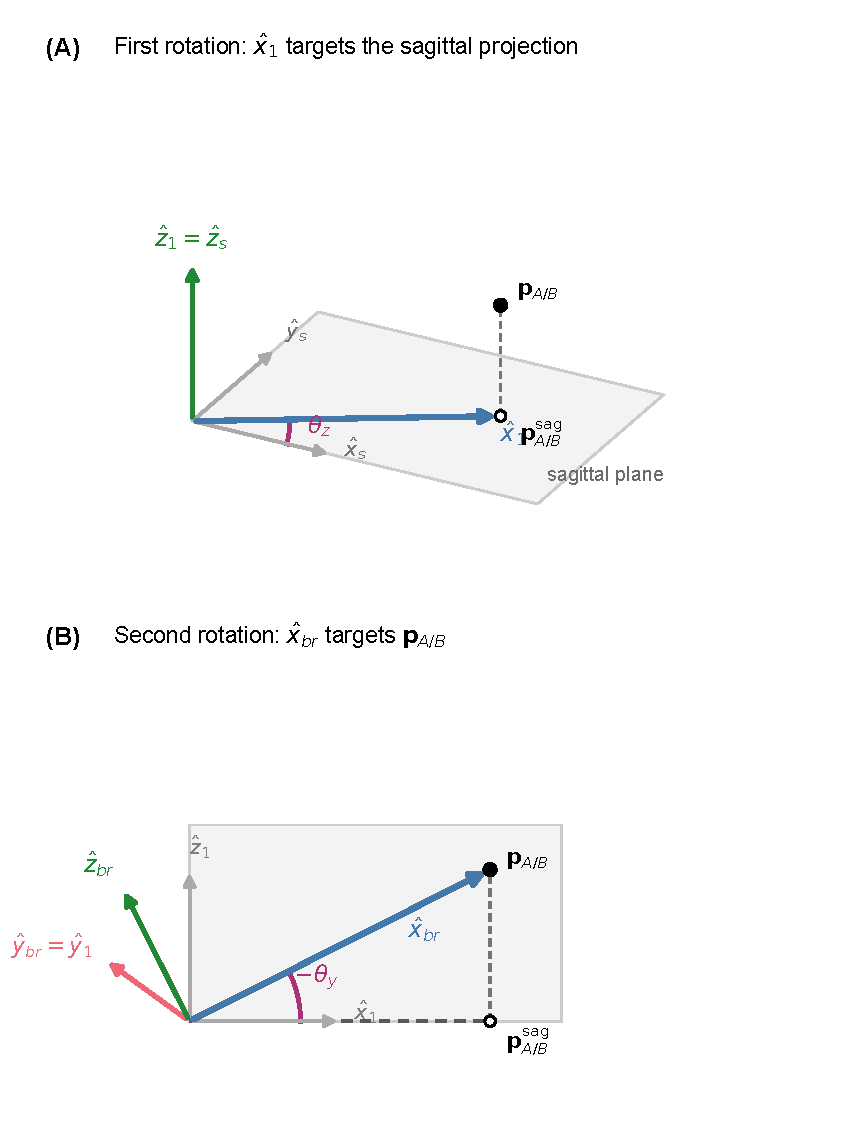
\includegraphics[height=0.62\textheight]{Figures/xiFrameTransform.pdf}
\end{center}
\caption{Two-rotation construction of the bracket frame from the attachment point $\mathbf{p}_{A}$ or $\mathbf{p}_{B}$. \textbf{(A)} Rotation through $\theta_z$ about the fixed $\hat{\mathbf{z}}_{s}$ axis aligns the intermediate axis $\hat{\mathbf{x}}_{1}$ with the point's sagittal-plane projection. \textbf{(B)} Rotation through $-\theta_y$ about the current $\hat{\mathbf{y}}_{1}=\hat{\mathbf{y}}_{br}$ axis aligns the final bracket axis $\hat{\mathbf{x}}_{br}$ with the full point vector.}\label{fig:xiFrameTransform}
\end{figure}

\begin{figure}[H]
\begin{center}
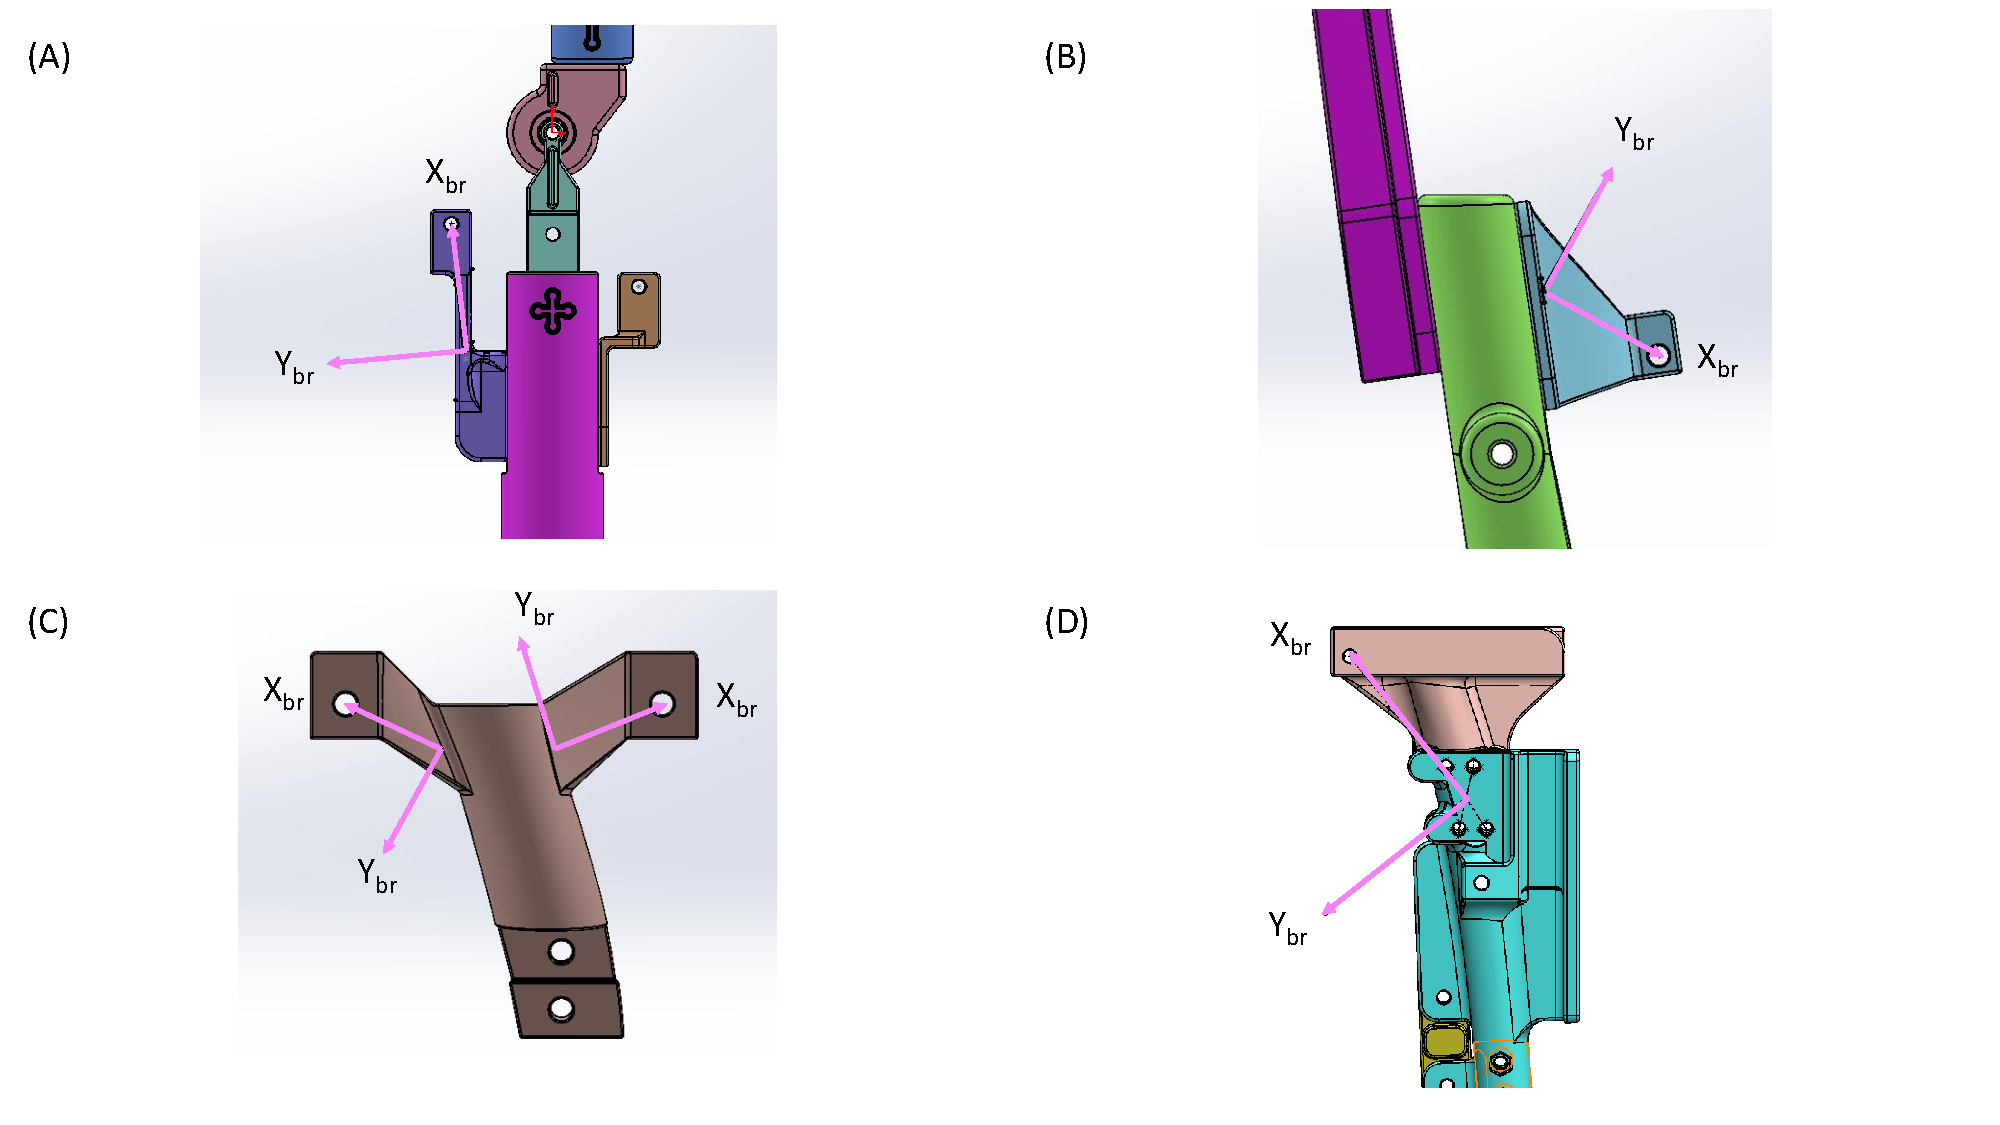
\includegraphics[width=1\textwidth]{Figures/bktFrame.pdf}
\end{center}
\caption{Bracket frame orientations for: \textbf{(A)} flexor configuration on the pinned knee, \textbf{(B)} extensor configuration on the pinned knee, \textbf{(C)} flexor and extensor configurations on the biomimetic knee with $\diameter$\qty{10}{\mm} BPAs, and \textbf{(D)} flexor configuration on the biomimetic knee with the $\diameter$\qty{20}{\mm} BPA.}\label{fig:bktFrame}
\end{figure}

In this frame the bracket is modeled as three independent linear springs, and the identified stiffness array is y-symmetric,
\begin{equation}
\mathbf{K}_{br} =
\begin{bmatrix}
\chi_{1} & 0   & 0 \\
0   & \chi_{2} & 0 \\
0   & 0   & \chi_{1} \\
\end{bmatrix}
\label{eq:bktstiffness}
\end{equation}
with $\chi_{1}$ the effective stiffness in the $x_{br}$ and $z_{br}$ directions and $\chi_{2}$ the effective bending stiffness along the cantilever direction $y_{br}$. The symmetry makes the compliance prediction independent of the frame convention: the pitch-only and two-rotation constructions of Figure~\ref{fig:xiFrameTransform} differ by a rotation about $\hat{\mathbf{y}}_{br}$, and a diagonal stiffness array is invariant under that rotation exactly when the two stiffnesses in its plane are equal.

Only the deflection component along the line of action changes the actuator's effective length. With the force in the bracket frame written $F\,\hat{\mathbf{u}}$, where $\hat{\mathbf{u}}$ is the BPA force direction, the deflection $\mathbf{K}_{br}^{-1}F\,\hat{\mathbf{u}}$ projects onto the line of action as
\begin{equation}
\delta_{br} = F\, \hat{\mathbf{u}}^{T} \, \mathbf{K}_{br}^{-1} \, \hat{\mathbf{u}}
\label{eq:bktprojectedcompliance}
\end{equation}
so the bracket presents the scalar stiffness
\begin{equation}
k_{\hat{u},br} = \frac{F}{\delta_{br}} = \left( \hat{\mathbf{u}}^{T} \mathbf{K}_{br}^{-1} \hat{\mathbf{u}} \right)^{-1}
\label{eq:keff}
\end{equation}
along the force path. An artificial tendon is modeled as an axial spring of stiffness $k_{ten} = n A_{c} E / L_{ten}$, with $n = 2$ parallel cable strands (six for the $\diameter$\qty{20}{\mm} assembly), cable cross-sectional area $A_{c} = \qty{1.51e-6}{\metre\squared}$, and modulus $E = \qty{193}{\giga\pascal}$. Bracket deflection and tendon stretch both shorten the effective BPA length under the same force, so their scalar compliances add in series:
\begin{equation} k_{eq} = \left( \frac{1}{k_{\hat{u},br}} + \frac{1}{k_{ten}} \right)^{-1}
\label{eq:equivalentstiffness}
\end{equation}

The compliance displacement shortens the actuator, so the active length entering the force model is
\begin{equation} l_m(\delta) = l_m^{(0)} - \delta
\label{eq:activelengthcorrected}
\end{equation}
where $l_m^{(0)}$ is the initial length of Equation~\eqref{eq:Lm}. Because the force depends on contraction, and the contraction on the compliance displacement, $\delta$ is the root of the implicit balance
\begin{equation} F_{620}(l_{0}) \, F^{*}\!\left(\varepsilon^*(\delta),P^*\right) - k_{eq}\,\delta = 0
\label{eq:complianceforcebalance}
\end{equation}
solved by bracketed scalar root-finding between zero deflection and the deflection that would bring the actuator to its maximum usable contraction, with $\delta = 0$ returned when the residual shows no sign change across that interval. The solved force gives the vector bracket deflection, which updates the attachment location; the routed length, force direction, moment arm, and torque are recalculated at the deflected geometry. The stiffness terms are effective parameters for the attachment system as a whole, absorbing the printed brackets, the bone fixtures, and the winch cable, and they are identified from torque rather than measured on any component in isolation.

Both ends of the actuator path can be compliant: the insertion-side bracket together with a second, origin-side bracket. Each bracket $j$ develops a three-dimensional deflection $\boldsymbol{\eta}_{br,j}$ along its local frame basis, of which only the projection along the corresponding force direction $\hat{\mathbf{u}}_j$ changes the actuator length, and the two projections act in series with the tendon elongation:
\begin{equation}
\begin{aligned}
\boldsymbol{\eta}_{br,j} &= \sum_{i=1}^{3}\eta_{i,j}\hat{\mathbf{e}}_i^{(j)},\\
\delta_{br,j} &= \hat{\mathbf{u}}_j^T\boldsymbol{\eta}_{br,j}, \qquad j\in\{1,2\},\\
\delta_{\mathrm{series}} &= \delta_{br,1}+\delta_{\mathrm{tendon}}+\delta_{br,2}.
\end{aligned}
\label{eq:bracket_series_projection}
\end{equation}

\subsection{Fictive Strain and Wrapping Loss}\label{sec:fictive_contraction}

The extensor configuration required one further correction, with a different physical origin than the compliance terms. As the knee flexes, the extensor BPA bends over the front of the joint, and part of the actuator follows the joint surface instead of a straight line. Bent this way, the BPA behaves like a beam: the pressurized wall on the inside of the bend carries less tension than the wall on the outside, and part of the wrapped arc length stops contributing usable contraction, so the actuator behaves as if it were more contracted than it physically is. We call this excess fictive strain: the additional contraction the force model must see to reproduce the observed force, beyond the actuator's physical contraction, expressed in $\varepsilon_{620}$-normalized units. A wrapping-loss term $\chi_{3}$ scales the length that this fictive strain removes:
\begin{equation}
    \Delta l = \begin{cases}
     \chi_{3}\;R\;\abs{ \theta_\text{wrap}-\theta_\text{k}}\;\zeta^2 & \theta_\text{k} \leq      \theta_\text{wrap} \\
      0 & \theta_\text{k} \geq      \theta_\text{wrap}
     \end{cases}\label{eq:deltaL}
\end{equation}
where $\Delta l$ is the change in usable length of the BPA, $R$ is the wrapping radius, $\abs{\theta_\text{wrap}-\theta_\text{k}}$ is the angle through which the BPA is bent once contact begins, and $\theta_\text{wrap}$, the knee flexion angle at which the BPA starts to bend over the joint, is determined from solid modeling. The factor $\zeta$ is the additive complement to the relative contraction,
\begin{equation}
    \zeta = 1-\varepsilon^*
\label{eq:comp}
\end{equation}
so the wrapping loss vanishes at full contraction and grows quadratically toward resting length. Combining Equations~\eqref{eq:comp} and~\eqref{eq:deltaL} with the offset of Equation~\eqref{eq:Lm} yields the fully corrected muscle length
\begin{equation}
    l_\text{m} = l_{LMT} - 2\;l_{fitting}  - \chi_{0} - \Delta l\label{eq:x3}
\end{equation}

\subsection{Identification Procedure}\label{sec:identification}

The correction terms enter the prediction through the implicit balance of Equation~\eqref{eq:complianceforcebalance}, and no instrument measures them directly, so they were identified by global optimization against measured torque. Candidates are judged simultaneously on the root mean square error (RMSE), the fraction of variance unexplained (FVU, the residual sum of squares divided by the total sum of squares of the measured torque about its mean, so that $R^{2} = 1 - \mathrm{FVU}$), and the maximum absolute residual, each computed between measured and predicted isometric torque over the tested range of motion; FVU is the primary criterion because it is scale-free and comparable across tests with different torque scales, while the maximum residual is the phase-sensitive worst case. The solver was an elitist nondominated-sorting genetic algorithm (gamultiobj in MATLAB, RRID:SCR\_001622) with adaptive-feasible mutation, scattered crossover at a fraction of 0.8, and a Pareto fraction of 0.35; each member of the returned Pareto front is scored on the reserved validation test, and the adopted solution is the member whose validation goodness of fit lies closest to its training-set fit. Where a family of members validates nearly equally well, as the flexor stiffness pairs do, the external redesign requirement of Section~\ref{sec:route_redesign_results} selects among them.

The identification proceeded in two stages. The flexor stage fits the two-bracket model $(\chi_{0}, \chi_{1}, \chi_{2})$ across the four pinned-knee flexor tests, with the $l_{0}=\qty{48.5}{\cm}$ and \qty{41.0}{\cm} tests in training and the $l_{0}=\qty{45.7}{\cm}$ and \qty{40.6}{\cm} tendon tests held out for validation. It evolved a population of 150 for up to 600 generations, terminating early once the relative change in the spread of the Pareto front fell below $4\times10^{-3}$. The extensor stage locks $(\chi_{1}, \chi_{2})$ to a member of the flexor Pareto front, enforcing a single stiffness pair across configurations, and solves only the extensor-specific terms $(\chi_{0}, \chi_{3})$ on a six-test pool of the pinned-extensor campaign, at resting lengths of \qty{40.0}{\cm} plain and with tendon, \qty{43.6}{\cm}, \qty{43.2}{\cm} with tendon, \qty{45.7}{\cm}, and \qty{46.5}{\cm}, with the \qty{43.6}{\cm}, \qty{43.2}{\cm}-tendon, and \qty{45.7}{\cm} tests in training and the \qty{40.0}{\cm} plain, \qty{40.0}{\cm}-tendon, and \qty{46.5}{\cm} tests held out for validation, and the extensor offset allowed negative values. The refit used a population of 50 for up to 150 generations at a spread tolerance of $1\times10^{-3}$. Both stages searched a normalized space, with length offsets in centimeters and stiffnesses on a base-ten logarithmic scale, so that the genetic search samples the decade-spanning stiffness bounds uniformly. The flexor bounds were $\chi_{0} \in [0, 20]$~\si{\milli\metre}, $\chi_{1} \in [3\times10^{4}, 10^{6}]$~\si{\N\per\metre}, and $\chi_{2} \in [5\times10^{3}, 2\times10^{4}]$~\si{\N\per\metre}; the extensor refit searched $\chi_{0} \in [-20, +5]$~\si{\milli\metre} and $\chi_{3} \in [0, 1]$ with the stiffness pair locked. The initial flexor population was drawn from $\chi_{0} \in [5, 15]$~\si{\milli\metre}, $\chi_{1} \in [5\times10^{4}, 5\times10^{5}]$, and $\chi_{2} \in [7\times10^{3}, 1.5\times10^{4}]$~\si{\N\per\metre}. An initial single-bracket identification, produced with the same framework before the origin-side bracket was added, is reported alongside the results figures; the two-stage procedure superseded it, and its adopted values are given in the Discussion.

\subsection{Route-Redesign Procedure}\label{sec:route_redesign}

With the correction terms fixed, the attachment routes themselves become design variables, and their best values are the ones that make the redesigned routes meet or exceed human knee torque capability. The redesign was carried out on the robot-body model derived from the Gait2392 lower-extremity model \citep{delp_opensim_2007,seth_opensim_2018}. The human targets are maximum-isometric torque curves: OpenSim moment arms, the partial derivative of muscle-tendon length with respect to the knee coordinate, $r(\theta_{k}) = \partial l_{\mathrm{MT}}/\partial\theta_{k}$, multiplied by each muscle's maximum isometric force \citep{delp_interactive_1990,hoy_musculoskeletal_1990,yamaguchi_planar_1989,sherman_what_2013,millard_flexing_2013,thelen_adjustment_2003,seth_opensim_2011}. The extensor is graded against vastus medialis and the flexor against biceps femoris short head; each target carries a required margin of 5\,\% above the human curve, so a route that merely touches the target at any angle is rejected.

The design variables are the BPA origin $\mathbf{p}_{1}$, the insertion $\mathbf{p}_{\mathrm{end}}$, the resting length, and the tendon length. Because the route prediction (contact activation, wrapping, and the compliance correction) is expensive to evaluate and only moderately smooth, the redesign minimizes a scalar cost assembled from weighted penalty terms:
\begin{equation}
    J = w_{w}\,J_{\text{worst}} + w_{t}\,J_{\text{torque}} + \textstyle\sum_{a} J_{a} + J_{\text{geom}} + J_{\text{len}}
    \label{eq:opt_cost}
\end{equation}
where $J_{\text{worst}}$ is the largest fraction by which robot torque falls short of the human target at any angle, weighted at $w_{w} = 10^{5}$, and $J_{\text{torque}}$ is the mean-squared shortfall fraction, weighted at $w_{t} = 10^{3}$, two orders of magnitude lower so that no single-angle shortfall can be traded for a better average. The $J_{a}$ are configuration-specific penalties (torque overshoot above the human curve, off-axis torque, wrap release), and $J_{\text{geom}}$ and $J_{\text{len}}$ regularize the endpoints and actuator lengths toward their seed values. Hard constraints, including bone clearance, wrap feasibility, actuator strain and contraction limits, and tendon geometry, reject failed candidates with a prohibitive penalty. The shared actuator plan is two $\diameter$\qty{20}{\mm} BPAs per route under a \qty{620}{\kPa} pressure ceiling, with a maximum usable contraction of 0.255 in the force model: the flexor model carries its two actuators on two separately solved routes, the second derived from the first by a mirrored distal attachment, with the two actuator forces summed, and the extensor model scales the force of a single shared route by the actuator count. Adjacent routes are required to maintain \qty{25}{\mm} of clearance.

Each run began with a sanity evaluation of the seed design, then executed a surrogate-assisted global solver under per-configuration evaluation budgets of 3,000 evaluations for the extensor route and 1,000 for the flexor route, and finally refined the best feasible point with a derivative-free mesh-adaptive pattern search for 15,000 further evaluations. The surrogate budgets cap run time rather than define convergence; the pattern search stops on its budget or early, once its mesh collapses with the constraints satisfied.

Three variants extend the search space. In the cam variant, the tibial-side route points trace a cam profile, so the routing geometry itself is shaped rather than only its endpoints. The pulley variants make the transmission ratio itself a design variable: a reeved tackle divides the force delivered at the insertion by its number of moving line parts $G$ and multiplies the insertion travel per unit of actuator contraction by the same factor, so the tackle converts surplus actuator force into range of motion, and the surplus is supplied by mounting BPAs in parallel or mirrored pairs, the same two-actuator-per-route arrangement the knee designs of this paper already use. With $n$ actuators in parallel feeding a tackle of $G$ line parts, the transmission's force gain is $n/G$ and its travel gain is $G$; for example, three actuators through a two-part tackle deliver 1.5 times the force of a single actuator at twice the travel. The mono-pulley variant reeves the tendon over a single tackle and serves uniarticular muscles, which cross one joint, and the bi-pulley variant reeves one tackle per joint crossed and serves biarticular and multi-articular muscles; the bi-pulley machinery was applied as a batch over five anatomical muscle sites of the robot-body model's leg. Every pulley run of record operated at unity transmission, the batch sites with one BPA and one line part per crossing and the mono-pulley flexor rig with its two actuators over a single line part, so no tackle altered the force or travel anywhere; the tendon exit followed the moving-force-point routing, fixed to the proximal body with the tendon direction recomputed as the joint rotates, rather than a bowden cable housing.


\section{Results}\label{sec:results_torque}

With the actuator force model characterized at the actuator level, we applied the same model to predict isometric torque about the knee on both test stands (Section~\ref{sec:robot_model}). In every configuration, the measured torque is compared against three predictions: the original rigid-body torque model, the improved BPA force characterization applied to the rigid kinematics, and the corrected torque model of Section~\ref{sec:improved_model} at its identified terms. The hybrid torque calculation (Section~\ref{sec:hybrid_method}) replaces the modeled muscle length and moment arm with their measured counterparts, which isolates kinematic error from force error. The coefficients quoted in this section are the initial single-bracket identification of Section~\ref{sec:identification}; the adopted two-stage values are reported in the Discussion. The two campaigns also reserve different validation tests: the initial flexor fit validated on the $l_{0}=\qty{45.7}{\cm}$ actuator and the two-stage flexor fit held out the $l_{0}=\qty{45.7}{\cm}$ and \qty{40.6}{\cm} tendon actuators, while the two-stage extensor pool holds out the $l_{0}=\qty{40.0}{\cm}$ plain, \qty{40.0}{\cm}-tendon, and \qty{46.5}{\cm} actuators.

\subsection{Flexor on Pin Joint}

Figure~\ref{fig:FlxPin_preopt} shows the measured flexor torque on the pinned knee next to the pre-optimization prediction series for the four cross-validation tests. Both pre-optimization force models overpredicted the magnitude of the measured flexor torque, and on the angles where the two predictions are both defined the improved BPA characterization fit the measurements better than the Hunt equation on every test, although it degraded near full extension, where the Hunt-equation prediction is undefined altogether (Table~\ref{tab:FlxPinPreGof}). The Hunt-equation prediction is undefined near full extension, where its modeled strain falls below zero, so the Hunt-equation and improved-characterization columns of the table are scored head-to-head on the measured points at which the Hunt equation is defined (75 of 90, 17 of 20, 14 of 19, and 15 of 22 points, in panel order), while the back-calculated torque is scored on all measured points; the four tests are the cross-validation tests of the adopted two-stage identification. The back-calculated (hybrid) torque reproduced the measurements closely, which localizes the misprediction to the modeled kinematics, the muscle length $l_\text{m}$ and the moment arm $r$, rather than to the force model.

The initial identification, fitted on the $l_{0}=\qty{48.5}{\cm}$ test, yielded a length offset $\chi_{0} = \qty{11.9}{\mm}$ and effective stiffnesses $\chi_{1} = \qty{102}{\kilo\newton\per\meter}$ and $\chi_{2} = \qty{10.6}{\kilo\newton\per\meter}$. The corrected model at these terms followed the measured torque across the range of motion, including the loss of torque near full extension that the rigid-body prediction did not produce, and Figure~\ref{fig:FlxPin_optimized} shows this corrected-family behavior at the adopted two-stage terms. The $l_{0}=\qty{45.7}{\cm}$ actuator, configured to operate over a different joint range of motion, served as the validation test of the initial fit; the corrected prediction reproduced the measured torque there without refitting. At these initial terms, the corrected prediction for the fitting test had a root-mean-square error (RMSE) of \qty{1.616}{\newton\meter}, a fraction of variance unexplained (FVU) of 0.0958, and a maximum absolute residual of \qty{3.2527}{\newton\meter}; validation on the held-out actuator gave \qty{2.1214}{\newton\meter}, 0.0878, and \qty{5.1690}{\newton\meter}, respectively.

\begin{figure}[H]
\begin{center}
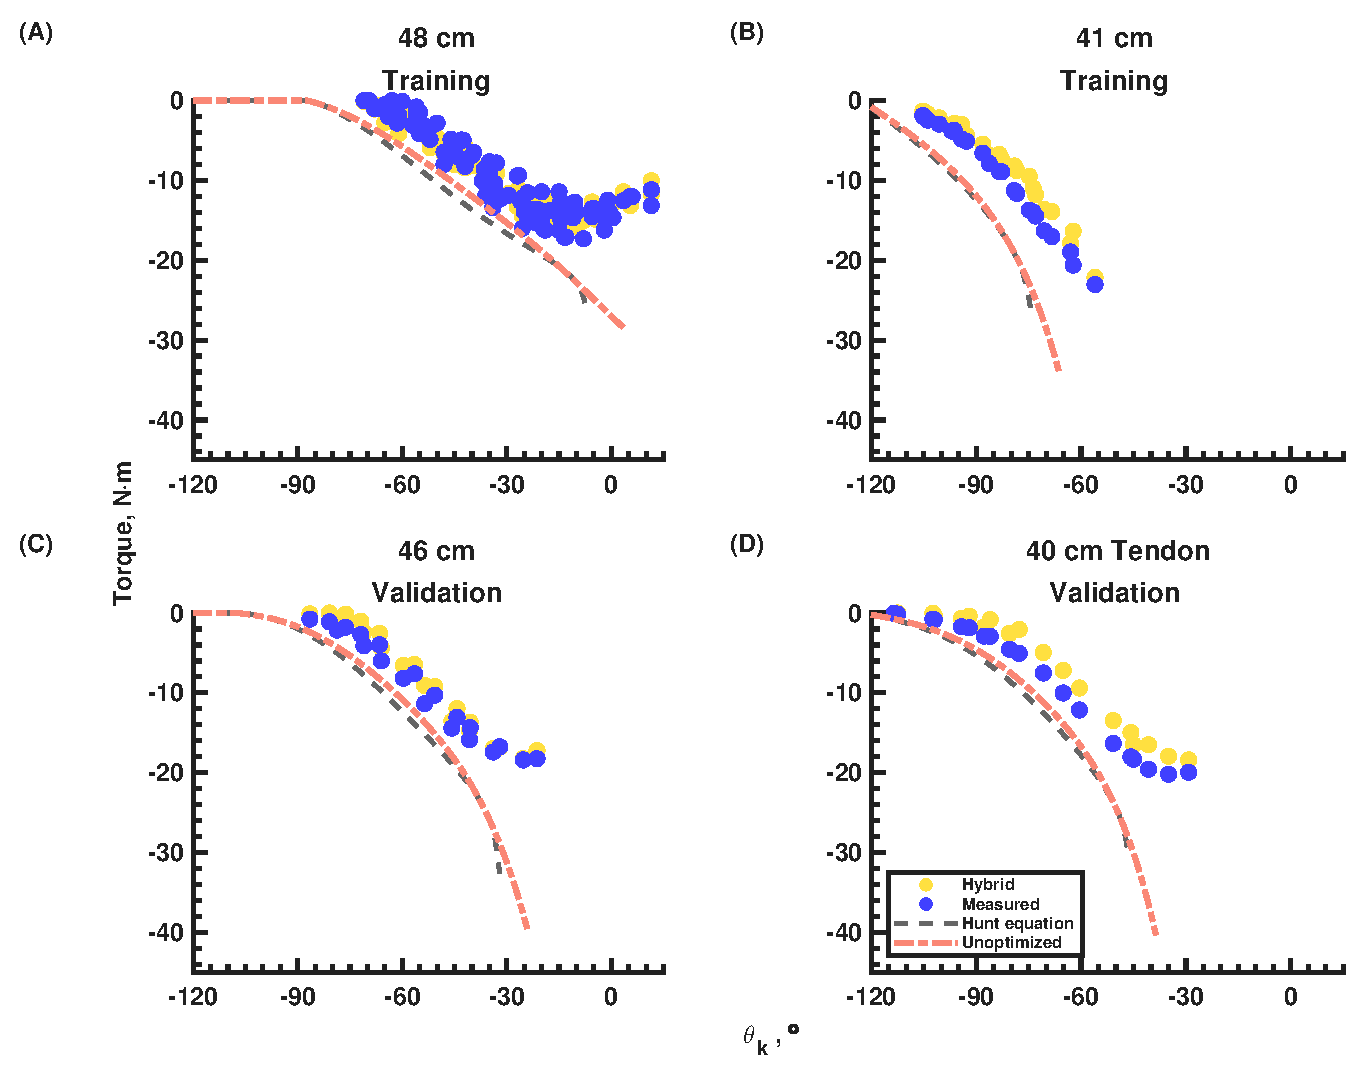
\includegraphics[width=0.8\textwidth]{Figures/FlxPin_preopt.eps}
\end{center}
\caption{Pre-optimization pinned-knee torque versus knee angle for the four cross-validation flexor tests. Knee angle is negative in flexion, and flexion torque is negative. Gold circles are the hybrid calculation; indigo filled circles are experimentally measured torque; the gray dashed line is the Hunt-equation rigid-body prediction; and the light orange dash-dot line is the unoptimized prediction, the improved BPA force characterization applied to the same rigid kinematics. Panel titles give the nominal resting length; the actual resting lengths $l_{0}$ are \textbf{(A)} \qty{48.5}{\cm}, \textbf{(B)} \qty{41.0}{\cm}, \textbf{(C)} \qty{45.7}{\cm}, and \textbf{(D)} \qty{40.6}{\cm} with tendon. Panels \textbf{(A)} and \textbf{(B)} are the training tests and panels \textbf{(C)} and \textbf{(D)} the validation tests of the adopted cross-validation fold.}\label{fig:FlxPin_preopt}
\end{figure}

\begin{table}[H]
\caption{Pre-optimization pinned-knee flexor torque-prediction goodness of fit per test, comparing the three pre-optimization torque predictions of Figure~\ref{fig:FlxPin_preopt}: the Hunt-equation rigid-body prediction, the unoptimized prediction of the improved BPA characterization, and the back-calculated (hybrid) torque. RMSE and maximum absolute residual (Max.) are in \unit{\newton\meter}, and FVU denotes the fraction of variance unexplained.}
\label{tab:FlxPinPreGof}
\begingroup
\renewcommand{\arraystretch}{1.4}%
\fontsize{10pt}{12pt}\selectfont
\begin{tabular}{@{}cc ccccccccc@{}}
\toprule
& & \multicolumn{3}{c}{\textbf{Hunt equation}} & \multicolumn{3}{c}{\textbf{Improved char.\ alone}} & \multicolumn{3}{c}{\textbf{Back-calculated (hybrid)}} \\
\cmidrule(lr){3-5} \cmidrule(lr){6-8} \cmidrule(l){9-11}
$\boldsymbol{l_{0}}$ (\unit{\cm}) & $\boldsymbol{l_{\text{ten}}}$ (\unit{\mm}) & \textbf{RMSE} & \textbf{FVU} & \textbf{Max.} & \textbf{RMSE} & \textbf{FVU} & \textbf{Max.} & \textbf{RMSE} & \textbf{FVU} & \textbf{Max.} \\
\midrule
48.5 & -- & 5.779 & 1.1761 & 9.798 & 4.871 & 0.8354 & 9.865 & 1.635 & 0.0991 & 3.842 \\
41.0 & -- & 6.633 & 3.2313 & 11.409 & 6.074 & 2.7090 & 9.262 & 2.187 & 0.1184 & 4.243 \\
45.7 & -- & 5.315 & 0.9408 & 9.991 & 4.465 & 0.6640 & 9.536 & 1.246 & 0.0409 & 2.275 \\
40.6 & 35 & 3.945 & 0.6750 & 7.527 & 3.226 & 0.4512 & 7.376 & 2.085 & 0.0755 & 3.073 \\
\bottomrule
\end{tabular}
\endgroup
\end{table}

\begin{figure}[H]
\begin{center}
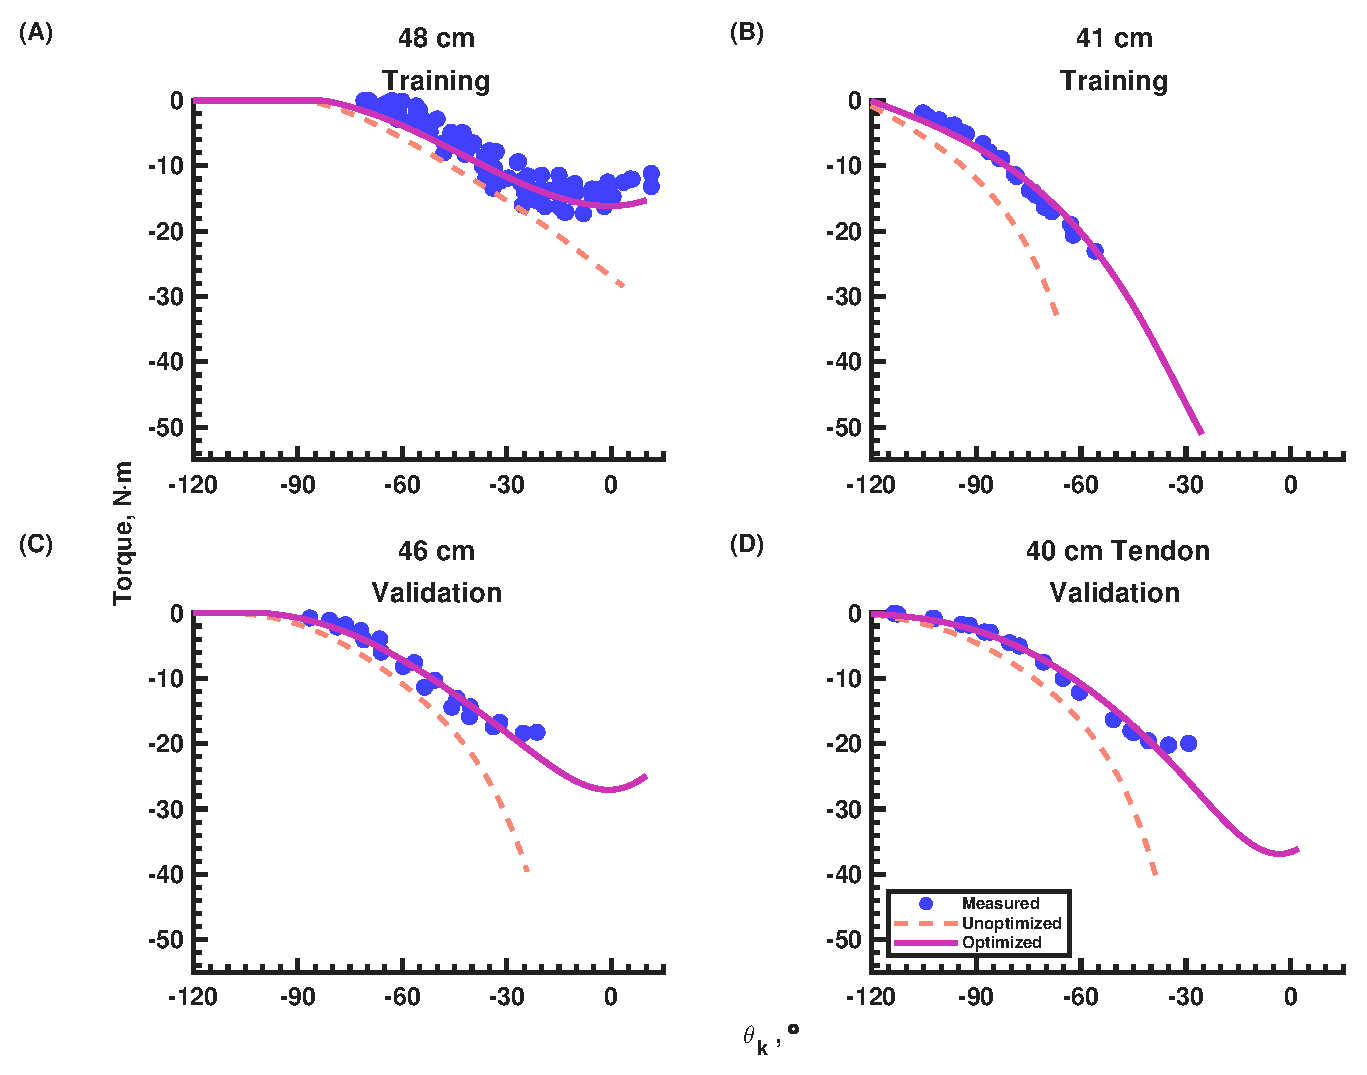
\includegraphics[width=0.8\textwidth]{Figures/FlxPin_optimized.eps}
\end{center}
\caption{Optimized pinned-knee torque versus knee angle for the four cross-validation flexor tests, at the adopted correction terms (Table~\ref{tab:AdoptedXi}). Knee angle is negative in flexion, and flexion torque is negative. Blue filled circles are experimentally measured torque; the dashed light orange line is the unoptimized prediction of the improved BPA characterization; the magenta line is the optimized prediction of the corrected model. Panel titles give the nominal resting length; the actual resting lengths $l_{0}$ are \textbf{(A)} \qty{48.5}{\cm}, \textbf{(B)} \qty{41.0}{\cm}, \textbf{(C)} \qty{45.7}{\cm}, and \textbf{(D)} \qty{40.6}{\cm} with tendon. Panels \textbf{(A)} and \textbf{(B)} are the training tests and panels \textbf{(C)} and \textbf{(D)} the validation tests of the adopted cross-validation fold; the goodness-of-fit values are given in Table~\ref{tab:FlxPinGof}.}\label{fig:FlxPin_optimized}
\end{figure}

\begin{table}[H]
\caption{Pinned-knee flexor torque-prediction goodness of fit: the improved BPA characterization alone (the zero-correction prediction of the text) and the corrected model at the adopted correction terms (Table~\ref{tab:AdoptedXi}); training and validation tests follow the adopted cross-validation fold. RMSE and maximum absolute residual (Max.) are in \unit{\newton\meter}, and FVU denotes the fraction of variance unexplained.}
\label{tab:FlxPinGof}
\begingroup
\renewcommand{\arraystretch}{1.4}%
\fontsize{10pt}{12pt}\selectfont
\begin{tabular}{@{}cc cccccc@{}}
\toprule
& & \multicolumn{3}{c}{\textbf{Improved BPA char.\ alone}} & \multicolumn{3}{c}{\textbf{Corrected model}} \\
\cmidrule(lr){3-5} \cmidrule(l){6-8}
$\boldsymbol{l_{0}}$ (\unit{\cm}) & $\boldsymbol{l_{\text{ten}}}$ (\unit{\mm}) & \textbf{RMSE} & \textbf{FVU} & \textbf{Max.} & \textbf{RMSE} & \textbf{FVU} & \textbf{Max.} \\
\midrule
\multicolumn{8}{@{}l}{\textbf{Training}} \\
48.5 & -- & 7.617 & 2.1278 & 25.531 & 2.165 & 0.1718 & 5.467 \\
41.0 & -- & 9.694 & 2.1149 & 21.076 & 1.084 & 0.0277 & 1.766 \\
\multicolumn{2}{@{}l}{\hspace*{1em}Mean} & 8.656 & 2.1213 & 23.303 & 1.624 & 0.0998 & 3.617 \\
\midrule
\multicolumn{8}{@{}l}{\textbf{Validation}} \\
45.7 & -- & 8.803 & 1.9380 & 26.264 & 1.368 & 0.0468 & 3.614 \\
40.6 & 35 & 6.373 & 0.5935 & 16.859 & 1.611 & 0.0427 & 5.891 \\
\multicolumn{2}{@{}l}{\hspace*{1em}Mean} & 7.588 & 1.2657 & 21.562 & 1.490 & 0.0447 & 4.752 \\
\bottomrule
\end{tabular}
\endgroup
\end{table}

\subsection{Extensor on Pin Joint}

Two features of the pinned-extensor measurements shaped the extensor identification. First, the measured torque crossed zero at a more extended angle than the prediction, indicating a length offset opposite in sign to the flexor offset. Second, on the $l_{0}=\qty{45.7}{\cm}$ test the hybrid calculation tracked the original prediction closely while the measured torque diverged from both, and the divergence grew with torque as the actuator wrapped over the joint.

The stiffness pair was held at the flexor-identified values, and the initial extensor identification added two extensor-specific terms: $\chi_{0} = \qty{-10.9}{\mm}$ and $\chi_{3} = 0.123$; the extensor length offset is close to the flexor offset in magnitude and opposite in sign. The two-stage extensor refit of Section~\ref{sec:identification} used a six-test pool drawn from the same campaign (Table~\ref{tab:ExtPinGof}), with the \qty{45.7}{\cm} test serving as a training test of the adopted fold; Figure~\ref{fig:ExtPin_group} shows the six pool tests at the adopted terms.

\begin{figure}[H]
\begin{center}
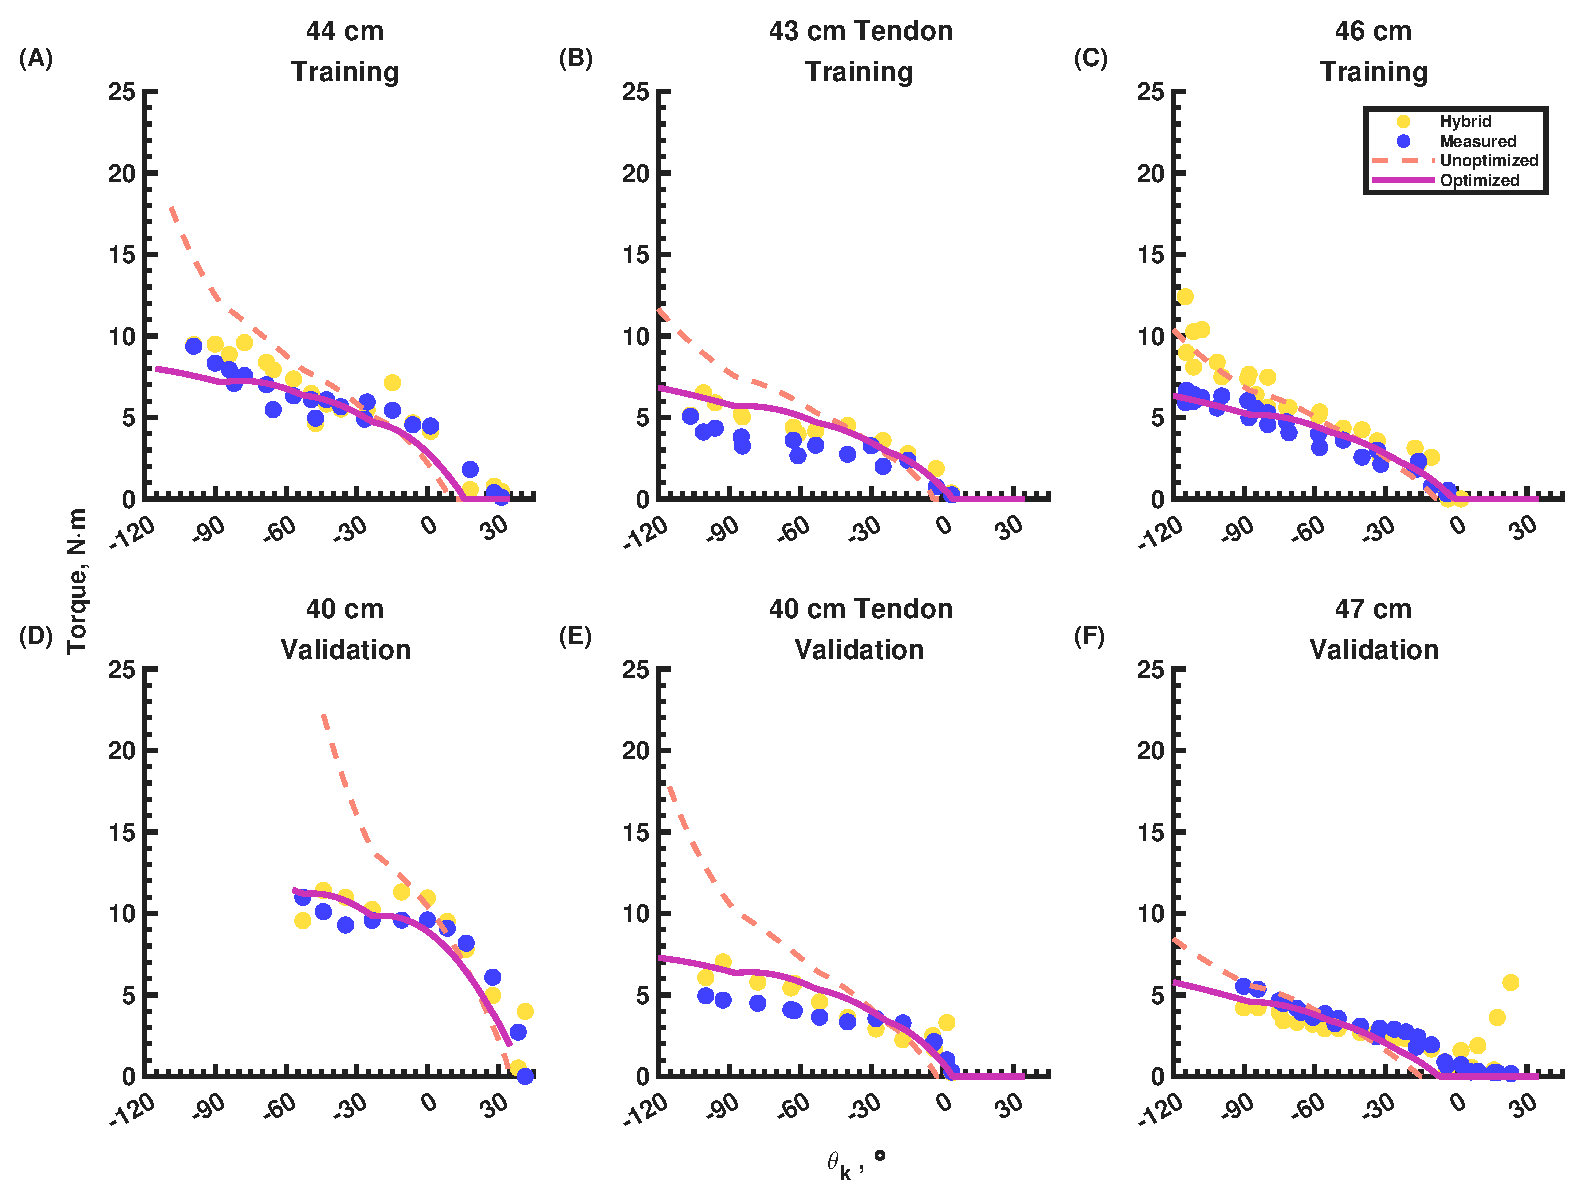
\includegraphics[width=1.0\textwidth]{Figures/ExtPin_group.eps}
\end{center}
\caption{Pinned-knee torque versus knee angle for the extensor BPAs: the six identification-pool tests at the adopted correction terms, with the extensor-specific terms $(\chi_{0}, \chi_{3})$ on the shared stiffness pair (Table~\ref{tab:AdoptedXi}). Knee angle is negative in flexion, and extension torque is positive. Gold circles are the hybrid calculation; indigo filled circles are experimentally measured torque; the dashed light orange line is the unoptimized prediction of the improved BPA characterization; the magenta line is the optimized prediction of the corrected model. Panel titles give the nominal resting length; the actual resting lengths $l_{0}$ are \textbf{(A)} \qty{43.6}{\cm}, \textbf{(B)} \qty{43.2}{\cm} with tendon, \textbf{(C)} \qty{45.7}{\cm}, \textbf{(D)} \qty{40.0}{\cm}, \textbf{(E)} \qty{40.0}{\cm} with tendon, and \textbf{(F)} \qty{46.5}{\cm}. Panels \textbf{(A)}--\textbf{(C)} are the training tests and panels \textbf{(D)}--\textbf{(F)} the held-out validation tests of the adopted cross-validation fold; the legend is given in panel \textbf{(A)}.}\label{fig:ExtPin_group}
\end{figure}

\begin{table}[H]
\caption{Pinned-knee extensor torque-prediction goodness of fit, at the adopted correction terms with the effective-stiffness pair locked to the flexor-identified values (Table~\ref{tab:AdoptedXi}): the improved BPA characterization alone (the zero-correction prediction of the text) and the corrected model. RMSE and maximum absolute residual (Max.) are in \unit{\newton\meter}, and FVU denotes the fraction of variance unexplained.}
\label{tab:ExtPinGof}
\begingroup
\renewcommand{\arraystretch}{1.4}%
\fontsize{10pt}{12pt}\selectfont
\begin{tabular}{@{}cc cccccc@{}}
\toprule
& & \multicolumn{3}{c}{\textbf{Improved BPA char.\ alone}} & \multicolumn{3}{c}{\textbf{Corrected model}} \\
\cmidrule(lr){3-5} \cmidrule(l){6-8}
$\boldsymbol{l_{0}}$ (\unit{\cm}) & $\boldsymbol{l_{\text{ten}}}$ (\unit{\mm}) & \textbf{RMSE} & \textbf{FVU} & \textbf{Max.} & \textbf{RMSE} & \textbf{FVU} & \textbf{Max.} \\
\midrule
\multicolumn{8}{@{}l}{\textbf{Training}} \\
43.6 & -- & 2.437 & 0.9618 & 4.284 & 0.978 & 0.1634 & 1.818 \\
43.2 & 22 & 2.878 & 4.7304 & 4.817 & 1.525 & 1.3270 & 2.481 \\
45.7 & -- & 2.178 & 1.0586 & 4.974 & 0.490 & 0.0535 & 1.206 \\
\multicolumn{2}{@{}l}{\hspace*{1em}Mean} & 2.498 & 2.2503 & 4.692 & 0.997 & 0.5146 & 1.835 \\
\midrule
\multicolumn{8}{@{}l}{\textbf{Validation}} \\
40.0 & -- & 3.092 & 0.5638 & 4.842 & 1.244 & 0.1303 & 2.196 \\
40.0 & 40 & 3.622 & 6.3919 & 7.845 & 1.350 & 0.8878 & 1.890 \\
46.5 & -- & 0.949 & 0.3152 & 2.272 & 0.699 & 0.1714 & 1.559 \\
\multicolumn{2}{@{}l}{\hspace*{1em}Mean} & 2.554 & 2.4236 & 4.986 & 1.098 & 0.3965 & 1.882 \\
\bottomrule
\end{tabular}
\endgroup
\end{table}

\subsection{Extensor on Biomimetic Knee}

We tested the extensor configuration on the biomimetic knee with a $\diameter$\qty{10}{\mm} BPA at $l_{0}=\qty{51.8}{\cm}$. The measured torque fell well below both the original prediction and the hybrid calculation (Figure~\ref{fig:Ext10mm_52cm}). Applying the extensor terms identified on the pinned knee improved the prediction: at the adopted two-stage terms, the corrected model reached an RMSE of \qty{1.1702}{\newton\meter}, an FVU of 0.6681, and a maximum absolute residual of \qty{2.2088}{\newton\meter}, against \qty{3.0322}{\newton\meter}, 4.4856, and \qty{5.5870}{\newton\meter} for the original rigid-body prediction. On this configuration the actuator path passes between the femoral condyles close to the instantaneous center of rotation, a geometry that is difficult to represent with the modeled path (Supplementary Figure~\ref{fig:passThru}).

\begin{figure}[H]
\begin{center}
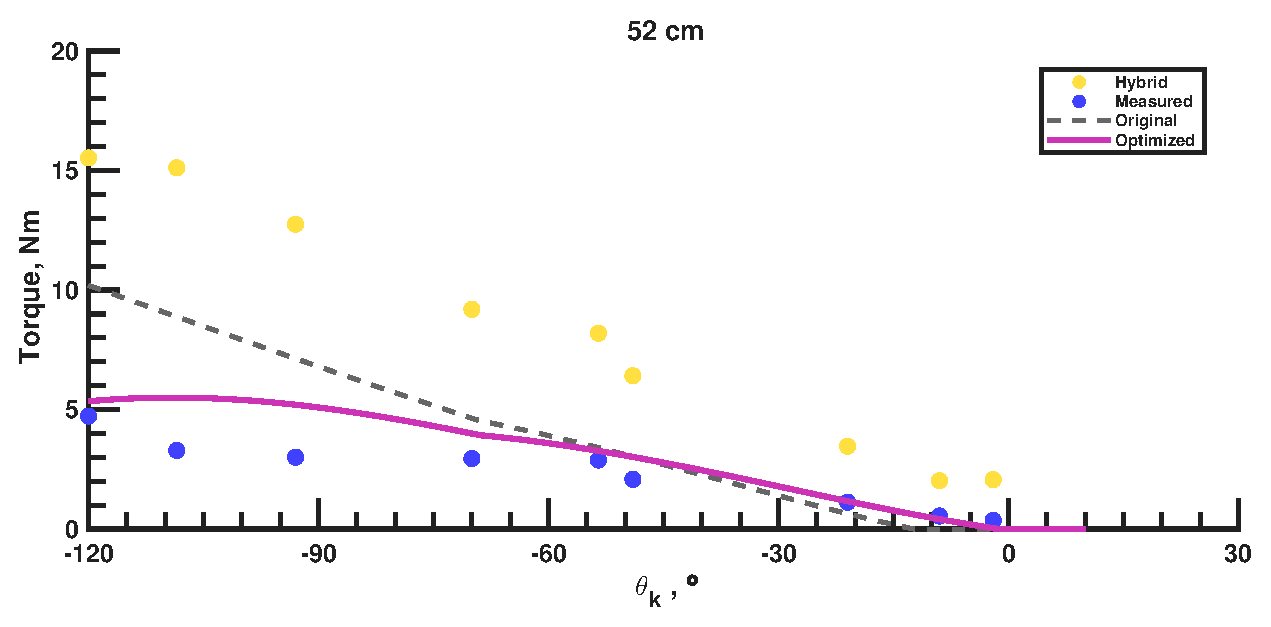
\includegraphics[width=0.75\textwidth]{Figures/Ext10mm_52cm.eps}
\end{center}
\caption{Biomimetic-knee torque versus knee angle for the $\diameter$\qty{10}{\mm}, $l_{0}=\qty{51.8}{\cm}$ extensor BPA. Knee angle is negative in flexion, and extension torque is positive. Indigo filled circles are experimentally measured torque; gold circles are the hybrid calculation; the gray dashed line is the original rigid-body prediction; the magenta line is the optimized prediction of the corrected model using the extensor terms identified on the pinned knee.}\label{fig:Ext10mm_52cm}
\end{figure}

\subsection{Flexor on Biomimetic Knee}

Figure~\ref{fig:FlxGrp} shows the biomimetic-knee flexor measurements with the flexor terms carried over unchanged from the pinned-knee identification. Panel \textbf{A} presents the $\diameter$\qty{10}{\mm} actuator at $l_{0}=\qty{41.5}{\cm}$ with a \qty{21}{\mm} artificial tendon ($\diameter$\qty{1.5}{\mm} bicycle brake cable wrapped four times), pressurized to \qty{604}{\kPa}; the corrected model reached an RMSE of \qty{0.3007}{\newton\meter}, an FVU of 0.0102, and a maximum absolute residual of \qty{0.4647}{\newton\meter}. Panel \textbf{B} presents the $\diameter$\qty{20}{\mm} actuator at $l_{0}=\qty{41.5}{\cm}$ with a \qty{14}{\mm} artificial tendon at \qty{620}{\kPa}, for which the corrected model reached an RMSE of \qty{1.8024}{\newton\meter}, an FVU of 0.0499, and a maximum absolute residual of \qty{3.5678}{\newton\meter}.

The torque of the single $\diameter$\qty{20}{\mm} flexor actuator of panel \textbf{B} did not exceed the magnitude of the maximum human isometric flexion torque \citep{delp_interactive_1990,seth_opensim_2018} between \ang{60} and \ang{100} of knee flexion; within a $\pm 20\%$ band about the human mean, it still fell short of human-level torque between \ang{78} and \ang{103} of flexion, the shortfall extending slightly past the upper end of the no-tolerance comparison. Because operating at \qty{620}{\kPa} across the full desired range of motion would load the printed femur beyond its ultimate strength, we also recorded single points at the reduced pressures \qtylist{560;421;325;281}{\kPa}, which show that the desired range of motion is achievable at reduced pressure. This shortfall in flexion torque defines the target that the attachment-route redesign reported in the Discussion addresses.

\begin{figure}[H]
\begin{center}
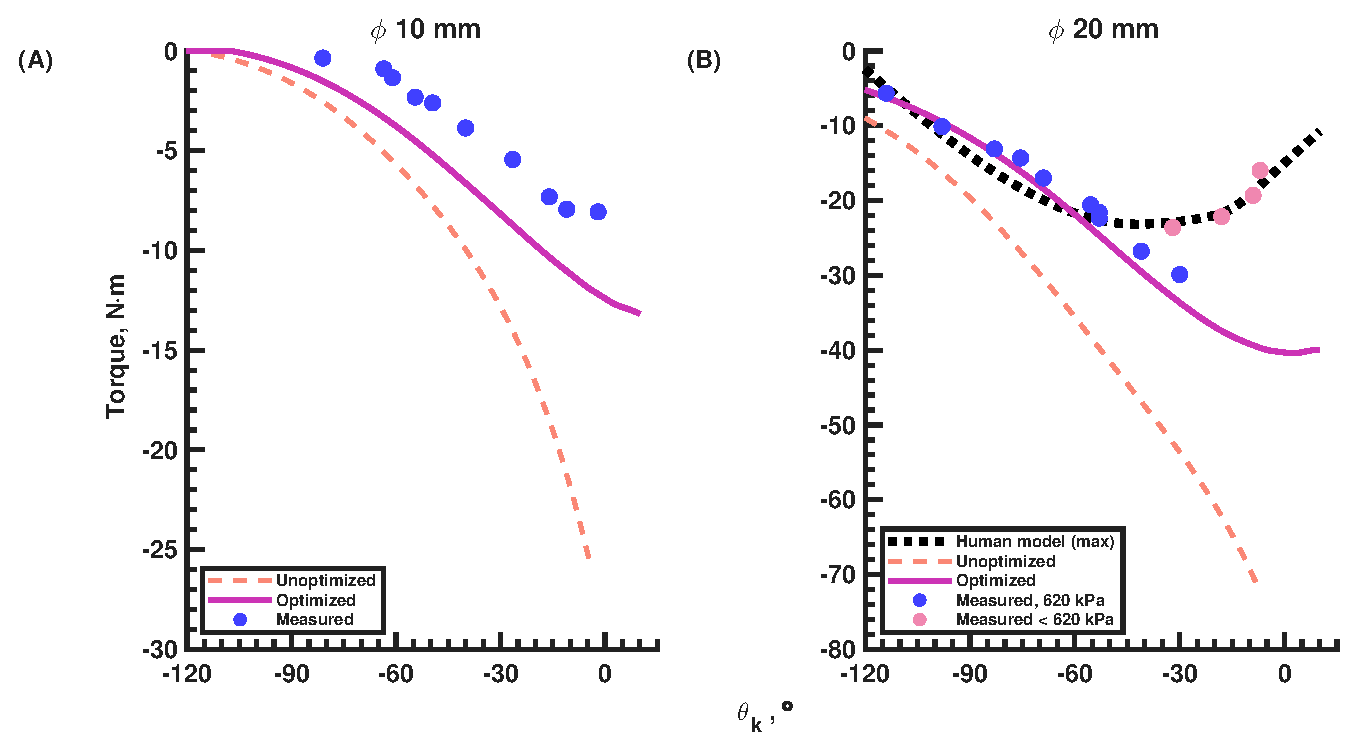
\includegraphics[width=0.9\textwidth]{Figures/FlxGrp.eps}
\end{center}
\caption{Biomimetic-knee torque versus knee angle for the flexor BPAs. Knee angle is negative in flexion, and flexion torque is negative. \textbf{(A)} $\diameter$\qty{10}{\mm}, $l_{0}=\qty{41.5}{\cm}$ actuator with a \qty{21}{\mm} artificial tendon at \qty{604}{\kPa}. \textbf{(B)} $\diameter$\qty{20}{\mm}, $l_{0}=\qty{41.5}{\cm}$ actuator with a \qty{14}{\mm} artificial tendon at \qty{620}{\kPa}. Indigo filled circles are measured torque; the magenta line is the optimized prediction of the corrected model using the flexor terms identified on the pinned knee; the dashed light orange line is the unoptimized prediction of the improved BPA characterization alone. In \textbf{(B)}, the black dotted line is the maximum human isometric torque, and the pink circles are measured points at the reduced pressures \qtylist{560;421;325;281}{\kPa}, recorded because full pressure would load the printed femur beyond its ultimate strength.}\label{fig:FlxGrp}
\end{figure}


\clearpage
\section{Discussion}\label{sec:discussion}

\subsection{Sources of Error in Isometric Torque Generation}\label{sec:disc_error}

The improved BPA force characterization removes part of the torque-prediction error, but only part (Figure~\ref{fig:FlxPin_preopt}). The remainder traces to the test system itself. The isometric system is not rigid: the winch cable, the artificial tendons, and the attachment brackets all bend and stretch under load, and the correction family $\chi_{0}$, $\chi_{1}$, and $\chi_{2}$ was created to represent them. Positioning tolerances, imperfect path modeling, and variation between individual actuators contribute as well.

The modeling of extensor paths that wrap around the knee is an approximation with inherent error, and the test-stand geometry amplifies it. When the moment arm is short, small changes to it have a large effect on the resultant torque \citep{young_analyzing_2019}, which is why moment-arm determination receives so much attention in musculoskeletal modeling \citep{brand_model_1982, menegaldo_moment_2004, suderman_moving_2012}. We chose to wrap the BPA around the joint rather than add a patella with a deterministically designed location and friction; the resulting path, which passes between the femoral condyles close to the migrating center of rotation of the biomimetic knee \citep{steele_biomimetic_2018}, resists any straight-line idealization (Supplementary Figure~\ref{fig:passThru}). At high flexion, the shorter actuators were also observed to stretch and compress (Figure~\ref{fig:testJigs}\textbf{C}), and the same loading occasionally slipped the actuator off the anterior bolt head that holds the femur to the knee, displacing the path by up to $\pm$\qty{20}{\mm} in the $Z$ direction and changing both the force vector and the torque.

The pinned extensor tests exposed one further error source, with a signature distinct from compliance. Figure~\ref{fig:ExtPin_group} shows a deviation between measured and originally predicted torque that widens as the expected torque grows, yet the hybrid calculation matches or exceeds the prediction except at the highest flexion angles. That combination points to a loss of functional muscle length rather than excess compliance, and it is why the wrapping-loss term $\chi_{3}$ was created in Equation~(\ref{eq:deltaL}). Bent over the joint, the actuator behaves like a beam, and the wrapped arc stops contributing usable contraction, so the actuator behaves as if it were more contracted than it physically is; this is the fictive strain of Section~\ref{sec:fictive_contraction}, and Section~\ref{sec:adopted_identification} quantifies it.

Working from the simple pinned knee to the complex biomimetic one isolated each of these mechanisms in turn. The products of that progression, a predictor for bending and axial compliance, a constant length offset, and a measure of the usable length lost as the actuator bends around a joint, are what make first-iteration torque design tractable for BPA-driven joints.

\subsection{Two-Stage Re-Identification and the Adopted Correction Terms}\label{sec:adopted_identification}

The coefficients quoted in the Results belong to the initial single-bracket identification (Section~\ref{sec:identification}). Re-identifying the correction terms over the full test sets, with the two-bracket flexor model and the locked extensor refit, yields the adopted values: $\chi_{0} = \qty{+3.94}{\mm}$, $\chi_{1} = \qty{3.998e4}{\N\per\m}$, and $\chi_{2} = \qty{1.473e4}{\N\per\m}$ for the flexor, and $\chi_{0} = \qty{-6.38}{\mm}$ with $\chi_{3} = 0.158$ for the extensor on the same locked stiffness pair (Table~\ref{tab:AdoptedXi}).

\begin{table}[H]
\caption{Adopted correction terms of the two-stage identification; the extensor refit locked the effective-stiffness pair $(\chi_{1}, \chi_{2})$ to the flexor-identified values, so one stiffness pair is shared across both configurations, and a dash marks a term not applied in that configuration. The stiffness terms are effective system stiffnesses that lump the compliance of the brackets, fixtures, and winch cable, and $\chi_{3}$ is unitless.}
\label{tab:AdoptedXi}
\begingroup
\renewcommand{\arraystretch}{1.4}%
\fontsize{10pt}{12pt}\selectfont
\begin{tabular}{@{}lccccc@{}}
\toprule
\textbf{Configuration} & $\boldsymbol{\chi_{0}}$ (\unit{\metre}) & $\boldsymbol{\chi_{1}}$ (\unit{\N\per\metre}) & $\boldsymbol{\chi_{2}}$ (\unit{\N\per\metre}) & $\boldsymbol{\chi_{3}}$ & $\boldsymbol{\chi_{4}}$ \\
\midrule
Flexor configuration & \num{+3.94e-3} & \num{3.998e4} & \num{1.473e4} & -- & -- \\
Extensor configuration & \num{-6.38e-3} & \num{3.998e4} & \num{1.473e4} & \num{0.158} & -- \\
\bottomrule
\end{tabular}
\endgroup
\end{table}

Each term has a direct physical reading. The offsets $\chi_{0}$ correct the effective muscle length by a constant, and the flexor and extensor offsets carry opposite signs, as the initial identification already showed. The stiffness pair is an effective system stiffness rather than the beam stiffness of any single part: it lumps the two attachment brackets together with the fixtures and the winch cable, which is why one pair can serve both configurations once the extensor refit locks it. The wrapping factor $\chi_{3}$ scales the usable length that fictive strain removes, $\Delta l = \chi_{3}\, R\, \abs{\theta_{\text{wrap}} - \theta_{\text{k}}}\, \zeta^{2}$ with $\zeta = 1 - \varepsilon^{*}$ (Equations~(\ref{eq:deltaL}) and (\ref{eq:comp})). Because $\varepsilon^{*}$ is normalized by the unloaded \qty{620}{\kPa} contraction $\varepsilon_{620}$ of the free actuator, the loss is expressed in fictive-contraction units: it vanishes as the actuator approaches full contraction, where $\zeta \to 0$, and grows quadratically toward resting length, exactly where a wrapped actuator has the least contraction to spare. The wrapping radii are fixed by the route geometry rather than fitted: the pinned-extensor identification evaluates two contact arcs of wrapping radii $R = \qty{12}{\mm}$ and $R = \qty{40}{\mm}$, and the biomimetic configurations use a wrap radius of \qty{25}{\mm}, so $\chi_{3} = 0.158$ scales a physical arc of known size.

Tables~\ref{tab:FlxPinGof} and \ref{tab:ExtPinGof} quantify what the corrections buy. On the pinned-flexor set, the corrected model reduces the training-mean RMSE, over the $l_{0}=\qty{48.5}{\cm}$ and \qty{41.0}{\cm} training tests, from \qty{8.66}{\newton\meter} to \qty{1.62}{\newton\meter} under the zero-correction prediction, the same kinematics and force model with every correction term disabled, and the validation mean over the held-out $l_{0}=\qty{45.7}{\cm}$ and \qty{40.6}{\cm} tendon tests improves from \qty{7.59}{\newton\meter} to \qty{1.49}{\newton\meter}; it holds the FVU at or below 0.172 on all four tests. On the extensor pool, the corrected model improves the RMSE of every test, reducing the training mean, over the \qty{43.6}{\cm}, \qty{43.2}{\cm}-tendon, and \qty{45.7}{\cm} tests, from \qty{2.50}{\newton\meter} to \qty{1.00}{\newton\meter}, and the validation mean, over the held-out \qty{40.0}{\cm} plain, \qty{40.0}{\cm}-tendon, and \qty{46.5}{\cm} tests, from \qty{2.55}{\newton\meter} to \qty{1.10}{\newton\meter}; the FVU stays below unity on every test except the $l_{0}=\qty{43.2}{\cm}$ tendon test. The biomimetic extensor test, a configuration held out of every identification, improves under the adopted two-stage terms as well: the corrected prediction reduces the RMSE from \qty{3.0322}{\newton\meter} to \qty{1.1702}{\newton\meter} and the FVU from 4.4856 to 0.6681 against the zero-correction baseline (Figure~\ref{fig:Ext10mm_52cm}). Evaluated at the initial single-bracket extensor terms instead, the corrected model reaches \qty{1.5394}{\newton\meter} and FVU 1.1560, so the adopted terms fit this held-out configuration more closely than the configuration-matched initial terms do.

The solver assignment follows the problem. The identification retains the genetic multiobjective solver, an elitist nondominated-sorting genetic algorithm, because the Pareto front it returns is what the holdout-validation procedure selects from. The route redesign is served by the surrogate-plus-pattern-search pipeline of Section~\ref{sec:route_redesign}, a surrogate-assisted global search refined by a derivative-free mesh-adaptive pattern search, because a single scalar cost is optimized there and each route evaluation is expensive.

The corrected force balance also admits an effective spring--damper reading in relative strain. Writing the quasistatic balance as the degenerate second-order system $m\,\ddot{\varepsilon}^{*} + c\,\dot{\varepsilon}^{*} + k(\varepsilon^{*}, P^{*})\,\varepsilon^{*} = F$, with local stiffness $k(\varepsilon^{*}, P^{*}) = \left.\partial F/\partial\varepsilon^{*}\right|_{P^{*}}$, and setting the mass and the external force of that analogy to zero leaves an effective damping $c = k\,\varepsilon^{*}/\dot{\varepsilon}^{*}$, which carries units of \unit{\newton\second\per\metre} because $\varepsilon^{*}$ is dimensionless. This is an interpretation of the quasistatic balance rather than a quantity this work measures: it states the ratio between the restoring force and the strain rate that the identification balances implicitly, and it connects the quasistatic corrections to the dynamic regime the robot leg will operate in, where the same compliance would set the joint's passive damping and a dynamic test could identify $c$ directly.

\subsection{Route Redesign Meeting Human Isometric Torque Targets}\label{sec:route_redesign_results}

The redesign addresses the single-actuator shortfall documented in the Results: one BPA per route does not reach the human flexor envelope through the mid-flexion range. Every redesigned configuration therefore carries two $\diameter$\qty{20}{\mm} BPAs per route, a \qty{620}{\kPa} pressure ceiling, and a maximum usable contraction of 0.255 in the force model, and every family was produced by the procedure of Section~\ref{sec:route_redesign} under the adopted correction terms of Table~\ref{tab:AdoptedXi}. The targets are maximum-isometric torque profiles computed on the Gait2392 lower-extremity model \citep{delp_opensim_2007, seth_opensim_2018}, the vastus medialis for the extensor and the biceps femoris short head for the flexor, each enlarged by a required \qty{5}{\percent} overshoot margin so that a route merely touching the target at any angle is rejected, and the redesign itself runs on the robot-body model derived from it. Knee angles are negative in flexion throughout this section, and Figure~\ref{fig:RouteVariants} graphs the four redesigned route families against their human-scaled requirements.

\begin{figure}[H]
\begin{center}
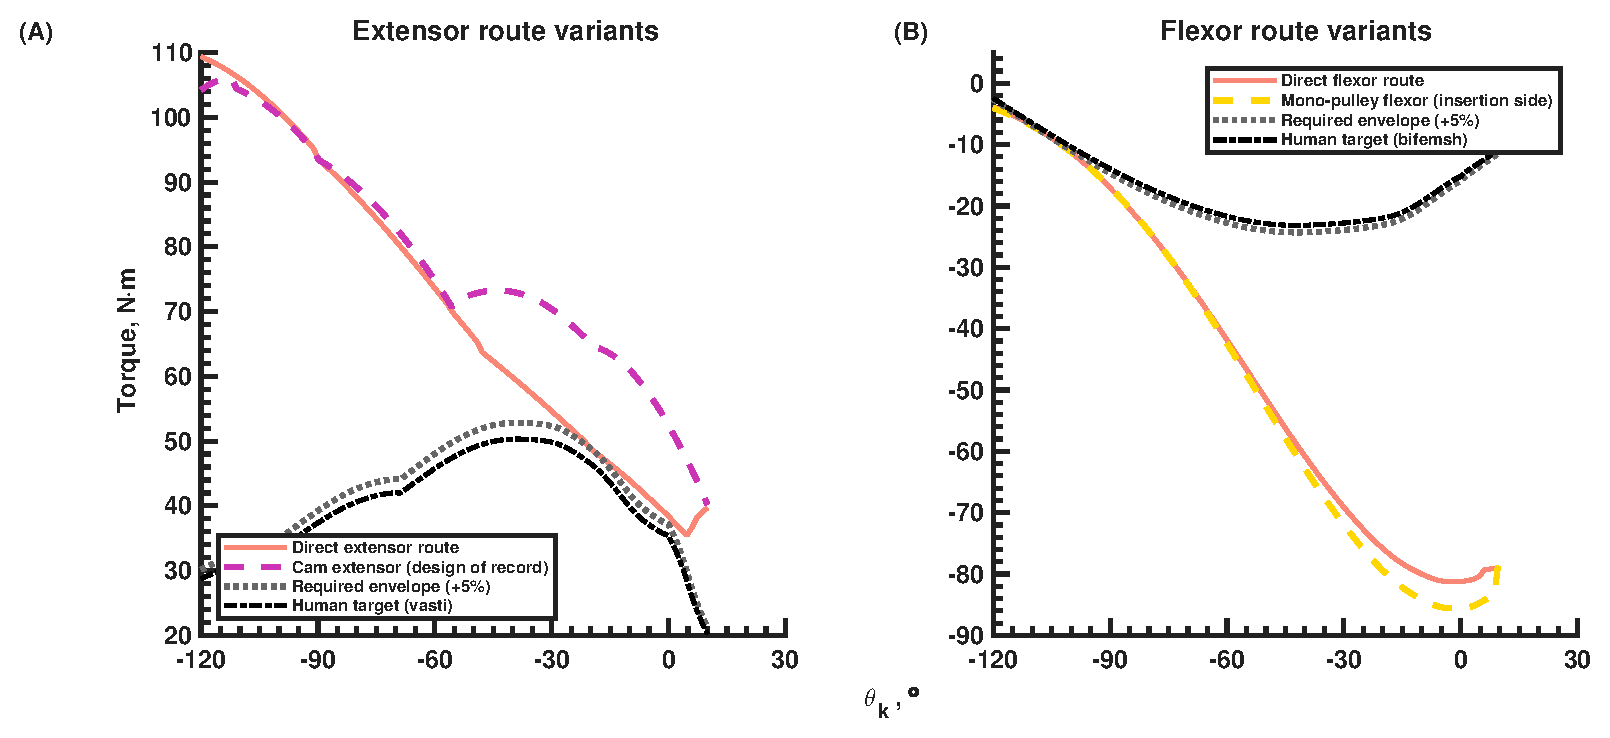
\includegraphics[width=1.0\textwidth]{Figures/RouteVariants_20261020.eps}
\end{center}
\caption{Predicted knee-axis torque of the redesigned route families against the human-scaled requirements. Knee angle is negative in flexion; extension torque is positive and flexion torque negative. \textbf{(A)} Extensor routes: the direct route and the cam design of record against the vasti requirement and its required \qty{5}{\percent} envelope. \textbf{(B)} Flexor routes: the direct two-BPA route and the mono-pulley variant on the insertion-side measure against the biceps femoris short-head requirement and its envelope.}\label{fig:RouteVariants}
\end{figure}

The direct extensor route exceeds the human envelope in magnitude at every angle, with zero shortfall points. Across the design range, the predicted two-BPA torque spans \qty{35.45}{\newton\meter} to \qty{109.4}{\newton\meter} against a human-scaled requirement of \qty{20.25}{\newton\meter} to \qty{50.32}{\newton\meter}, and the required overshoot is consumed as the thinnest margin exactly as designed, $+5.02$~\% at the worst-case angle of \ang{-20.2}. The route respects the wrap-release schedule of the route-elimination rule, releasing its six sequential contacts at knee angles of \ang{-89.8}, \ang{-55.7}, \ang{-47.8}, \ang{-20.2}, \ang{6.1}, and \ang{7.4}, and the optimized design places the femur-side origin at $(40.0, 137.0, 0)$~mm and the tibial insertion at $(34.4, -197.1, 0)$~mm, with a resting length of \qty{827.7}{\mm} and \qty{36.8}{\mm} of tendon.

\begin{figure}[H]
\begin{center}
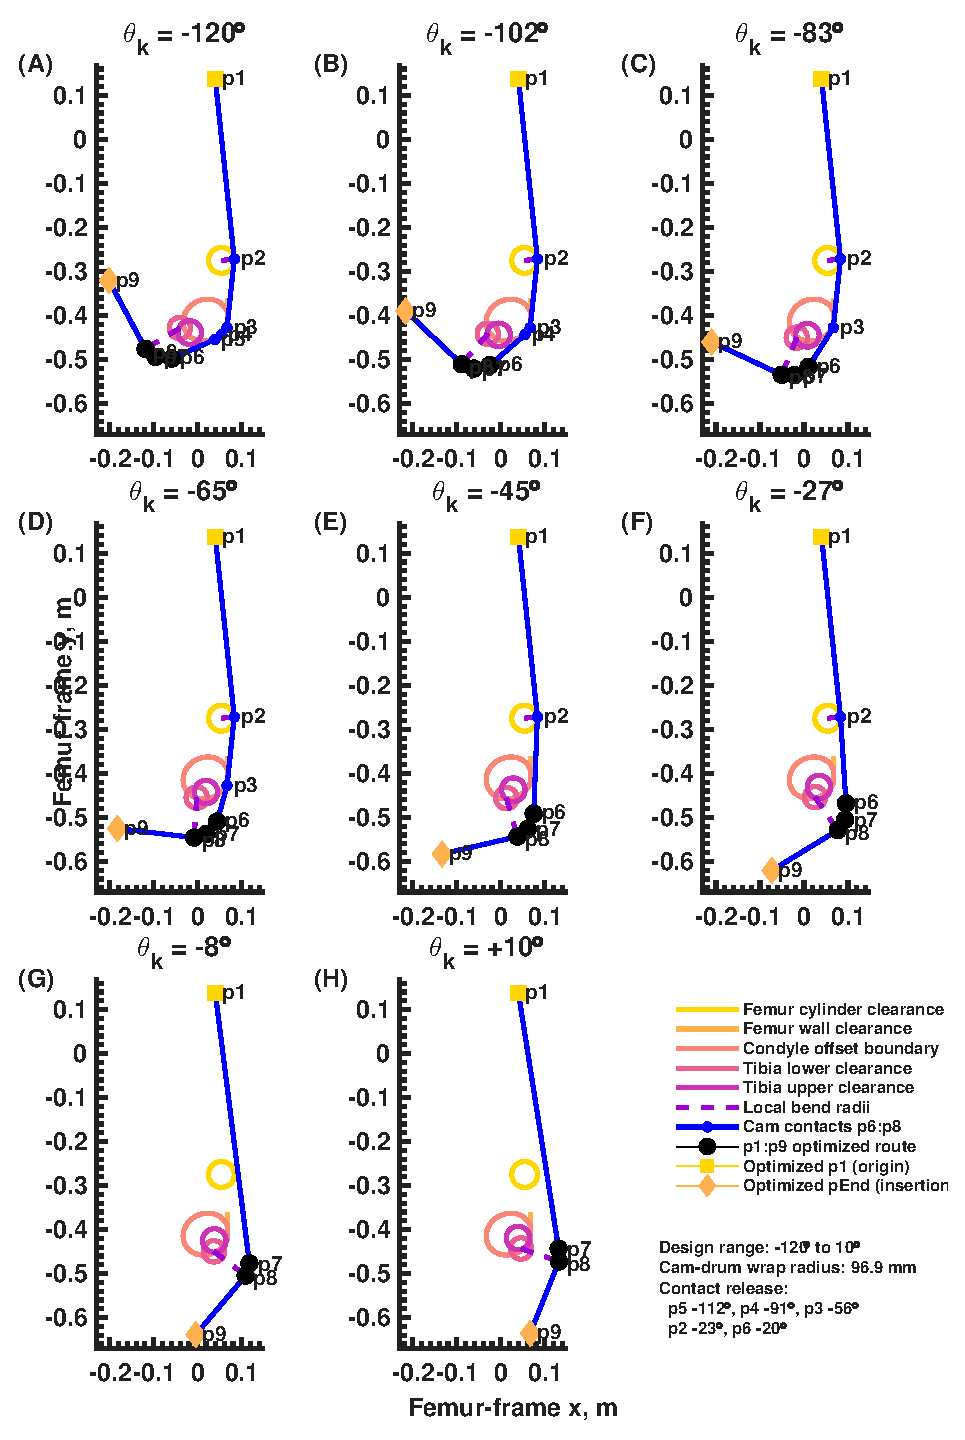
\includegraphics[width=1.0\textwidth]{Figures/ExtensorRoute_redesigned.eps}
\end{center}
\caption{Route geometry of the cam extensor design of record, drawn in the femur frame. Panels \textbf{(A)}--\textbf{(H)} show eight evenly spaced knee poses from full flexion ($\theta_\text{k} = \ang{-120}$) to full extension ($\theta_\text{k} = \ang{10}$); knee angle is negative in flexion. Each panel draws the optimized route and its cam contacts over the femur-cylinder, femur-wall, condyle, and tibia clearance envelopes of the route-elimination rule, with the local bend-radius checks dashed; the square marker is the femur-side origin, the diamond marker is the tibial insertion, and the ninth tile carries the legend and the contact-release schedule.}\label{fig:ExtensorRoute_redesigned}
\end{figure}

The extensor route was then redesigned once more by allowing the tibial-side route points to trace a cam profile, and this cam redesign is the current extensor design. The cam converts the razor-thin margin of the direct route into genuine headroom. On the final geometry, which folds the optimizer winner together with a verified adjustment of the distal route point and tendon length, the minimum torque margin is $+30.83$~\% with respect to the required envelope and $+39.77$~\% with respect to the plain human target; the unadjusted optimizer solution carried $+31.30$~\% and $+42.34$~\% at the same checks. The pressure required to meet the envelope spans \qty{269}{\kPa} to \qty{507}{\kPa} over the range of motion, comfortably above the \qty{150}{\kPa} regulated floor of the valve manifold that supplies the hardware, so the remaining pressure is a design resource. The geometry confirms that the headroom is not bought with routing risk: the tibial wrap follows a bend radius of \qty{96.9}{\mm}, the guiding route point clears the femoral-condyle envelope by \qty{43.1}{\mm} at \ang{10} of knee extension, and the moment arm spans \qty{59.4}{\mm} to \qty{102.8}{\mm} with a mean of \qty{72.4}{\mm} (Figure~\ref{fig:ExtensorRoute_redesigned}).

The flexor redesign is a two-BPA mirrored-route solution rather than a single shared route. The first actuator's route is carried directly as design variables, its origin on the femur and its insertion on the tibia, and the second actuator's endpoints are solved from it by a mirrored-endpoint rule: the second insertion mirrors the first across the mid-sagittal plane, and the second origin is placed so that the second route spans the same origin-to-insertion offset as the first, which keeps the two routes from crossing. Each route is then rebuilt by the route solver, so the second carries its own wrap point and its own tibial and femoral-condyle clearance state rather than inheriting the first's, with condyle clearance enforced in the nonlinear constraints. In the design of record the first route clears the tibial envelope at every angle and never wraps, while the second rides its standoff only within about \ang{5} of full extension before the wrap releases. The design meets the flexor target with a minimum margin fraction of 0.0501 against the required 0.05. Its predicted knee-axis torque spans \qty{-81.23}{\newton\meter} to \qty{-3.864}{\newton\meter} against the human-scaled requirement of \qty{-23.16}{\newton\meter} to \qty{-2.461}{\newton\meter} (peak magnitude \qty{23.16}{\newton\meter}), again exceeding the envelope at every angle. The flexor prediction applies the adopted correction terms, including the wrapping factor identified on the extensor configuration: where a route's wrap is active, the actuator loses usable length through the same wrapping mechanism, and the extensor-identified $\chi_{3}$ was applied to it unchanged, a transfer whose testing remains future work (Section~\ref{sec:limitations}).

The knee-flexor run quantifies what the mono-pulley freedom is worth at unity gain. As a uniarticular knee flexor, the biceps femoris short head is exactly the site the mono-pulley variant serves, and the run converged to a collision-feasible layout with zero bound violations, both actuators of the rig reeved over a single tackle of one line part, so the gain was 1 and no force multiplication was engaged; the run therefore measures the redirect baseline, not the transmission trade. Even the redirect alone deepened the peak predicted flexion torque from \qty{81.23}{\newton\meter} on the direct route to \qty{85.74}{\newton\meter} on the same knee-axis measure, \qty{85.56}{\newton\meter} on the insertion-side measure after the tackle's force loss, a gain of \qty{4.51}{\newton\meter} or \qty{5.6}{\percent}, while holding the off-axis torque to at most \qty{0.803}{\newton\meter}, under \qty{1}{\percent} of the peak. The direct and pulley runs optimize different objective functions, so their objective values, 74.47 and 0.08465, are not commensurable; the torque comparison, not the objective comparison, is the meaningful one. That comparison should still be read as the value of the added routing freedom in this pair of runs rather than as an isolated pulley effect, since no run at fixed objective separates the pulley's contribution. The predicted peaks of the direct and pulley routes exceed the human flexor scale of \qty{23.16}{\newton\meter} by factors of 3.51 and 3.70, and the torque-for-range exchange that a reeved tackle buys is quantified by the doctrine re-solves of the batch analysis that follows.

The bi-pulley machinery was then applied as a batch over five anatomical muscle sites of the robot-body model's leg, covering both halves of the pulley doctrine: three uniarticular sites that the mono-pulley variant serves, soleus and tibialis anterior at the ankle and biceps femoris short head at the knee, and two biarticular sites that the bi-pulley variant serves, medial gastrocnemius across the knee and ankle and rectus femoris across the hip and knee. Every run of record operated at unity transmission, one BPA and one tackle line part per crossing, with the tendon exit on the moving-force-point routing; the bowden-housing arrangement is implemented in the machinery but was never exercised. Because the point of a reeved tackle is to exchange actuator force for range of motion, each site was then re-solved in full at three doctrine configurations of the transmission: a parallel pair of BPAs through a two-part tackle (force gain 1, travel gain 2), the same pair through a four-part tackle (force gain 0.5, travel gain 4), and a four-actuator group through a four-part tackle (force gain 1, travel gain 4), all at supply pressures of \qtylist{300;450;620}{\kPa}. The actuator sizes are re-solved rather than carried over, because a route sized for direct drive runs its tendon slack under a multi-part tackle that feeds takeup faster than the span demands; the optimizer re-fits the actuator lengths to the transmission at every configuration. Figure~\ref{fig:PulleyTorqueSurfaces} shows the resulting torque surfaces over joint angle and pressure at the two-actuator, two-part configuration, and Figure~\ref{fig:PulleyMarginSurfaces} the margins against the human requirements over joint angle and the transmission ladder at \qty{620}{\kPa}. The human requirements are maximum-isometric torques of the stock Gait2392 model \citep{delp_opensim_2007, seth_opensim_2018}, computed as OpenSim moment arms times maximum isometric force (\qty{3549}{\N} soleus, \qty{905}{\N} tibialis anterior, \qty{1558}{\N} medial gastrocnemius, \qty{1169}{\N} rectus femoris), with the biceps femoris short head graded against the recorded human requirement of its own mono-pulley run, whose peak magnitude is \qty{23.16}{\newton\meter}.

The re-solves show the exchange operating in the direction the doctrine intends: at matched net force, the meeting range against the human requirement grows with the tackle's travel gain. The tibialis-anterior route is the strongest site: the single-actuator baseline meets the human dorsiflexor requirement, which spans \qtyrange{24.60}{39.35}{\newton\meter} over the ankle range, across \ang{48.1} of the \ang{70} ankle range (\ang{46.7} contiguous) at \qty{620}{\kPa} with a peak of \qty{52.0}{\newton\meter}, and its meeting range grows from zero at \qty{300}{\kPa} to \ang{14.6} at \qty{450}{\kPa} and \ang{48.1} at \qty{620}{\kPa}; the parallel pair through the two-part tackle holds the peak at \qty{53.0}{\newton\meter} and extends the meeting range to \ang{56.9} (\ang{55.4} contiguous), and the four-actuator group through the four-part tackle extends it further to \ang{59.8} (\ang{58.3} contiguous). At the knee, the biceps femoris short head is already served over its whole range by the direct two-actuator flexor redesign of Section~\ref{sec:route_redesign}, which exceeds the flexor requirement at every angle of the full \ang{130} span at a minimum margin fraction of 0.0501; the transmission study at this site therefore starts from the batch's unity-transmission single-actuator run, which meets its requirement only at isolated angles totaling \ang{5.4}, with eight of twenty-five grid cells infeasible at every pressure. Against that single-actuator baseline, the matched-force pair removes every infeasible cell and meets over \ang{27.1} of the span, and the four-actuator group reaches \ang{56.9} at a peak of \qty{25.9}{\newton\meter}; at this site the tackle's contribution is the multiplied insertion travel and the actuator-count scalability it buys, not meeting range that the direct design lacks. The medial gastrocnemius baseline meets over \ang{21.7} of the knee sweep with seven of twenty-five cells infeasible; the matched-force pair extends the meeting range to \ang{65.0}, and at force gain 0.5, with the pair alone feeding the four-part tackle, the design meets over \ang{105.6} of the sweep at a peak of \qty{118.0}{\newton\meter}, while the four-actuator group at matched force meets over \ang{119.2} at a peak of \qty{236.1}{\newton\meter}. The rectus femoris route was recorded with its knee crossing rigid, so its margins are evaluated over the hip angle, where the baseline meets over \ang{46.9} at \qty{620}{\kPa} and the matched-force pair more than doubles the meeting range to \ang{99.0}. The soleus site is the honest limit of the exchange: it never meets its human requirement at any transmission, a peak of \qty{25.3}{\newton\meter} against a required magnitude of \qtyrange{134.08}{171.35}{\newton\meter}, a factor of 6.8 short, because its shortfall is in force, and a tackle that divides force cannot add it, only the actuator count can.

\begin{figure}[H]
\begin{center}
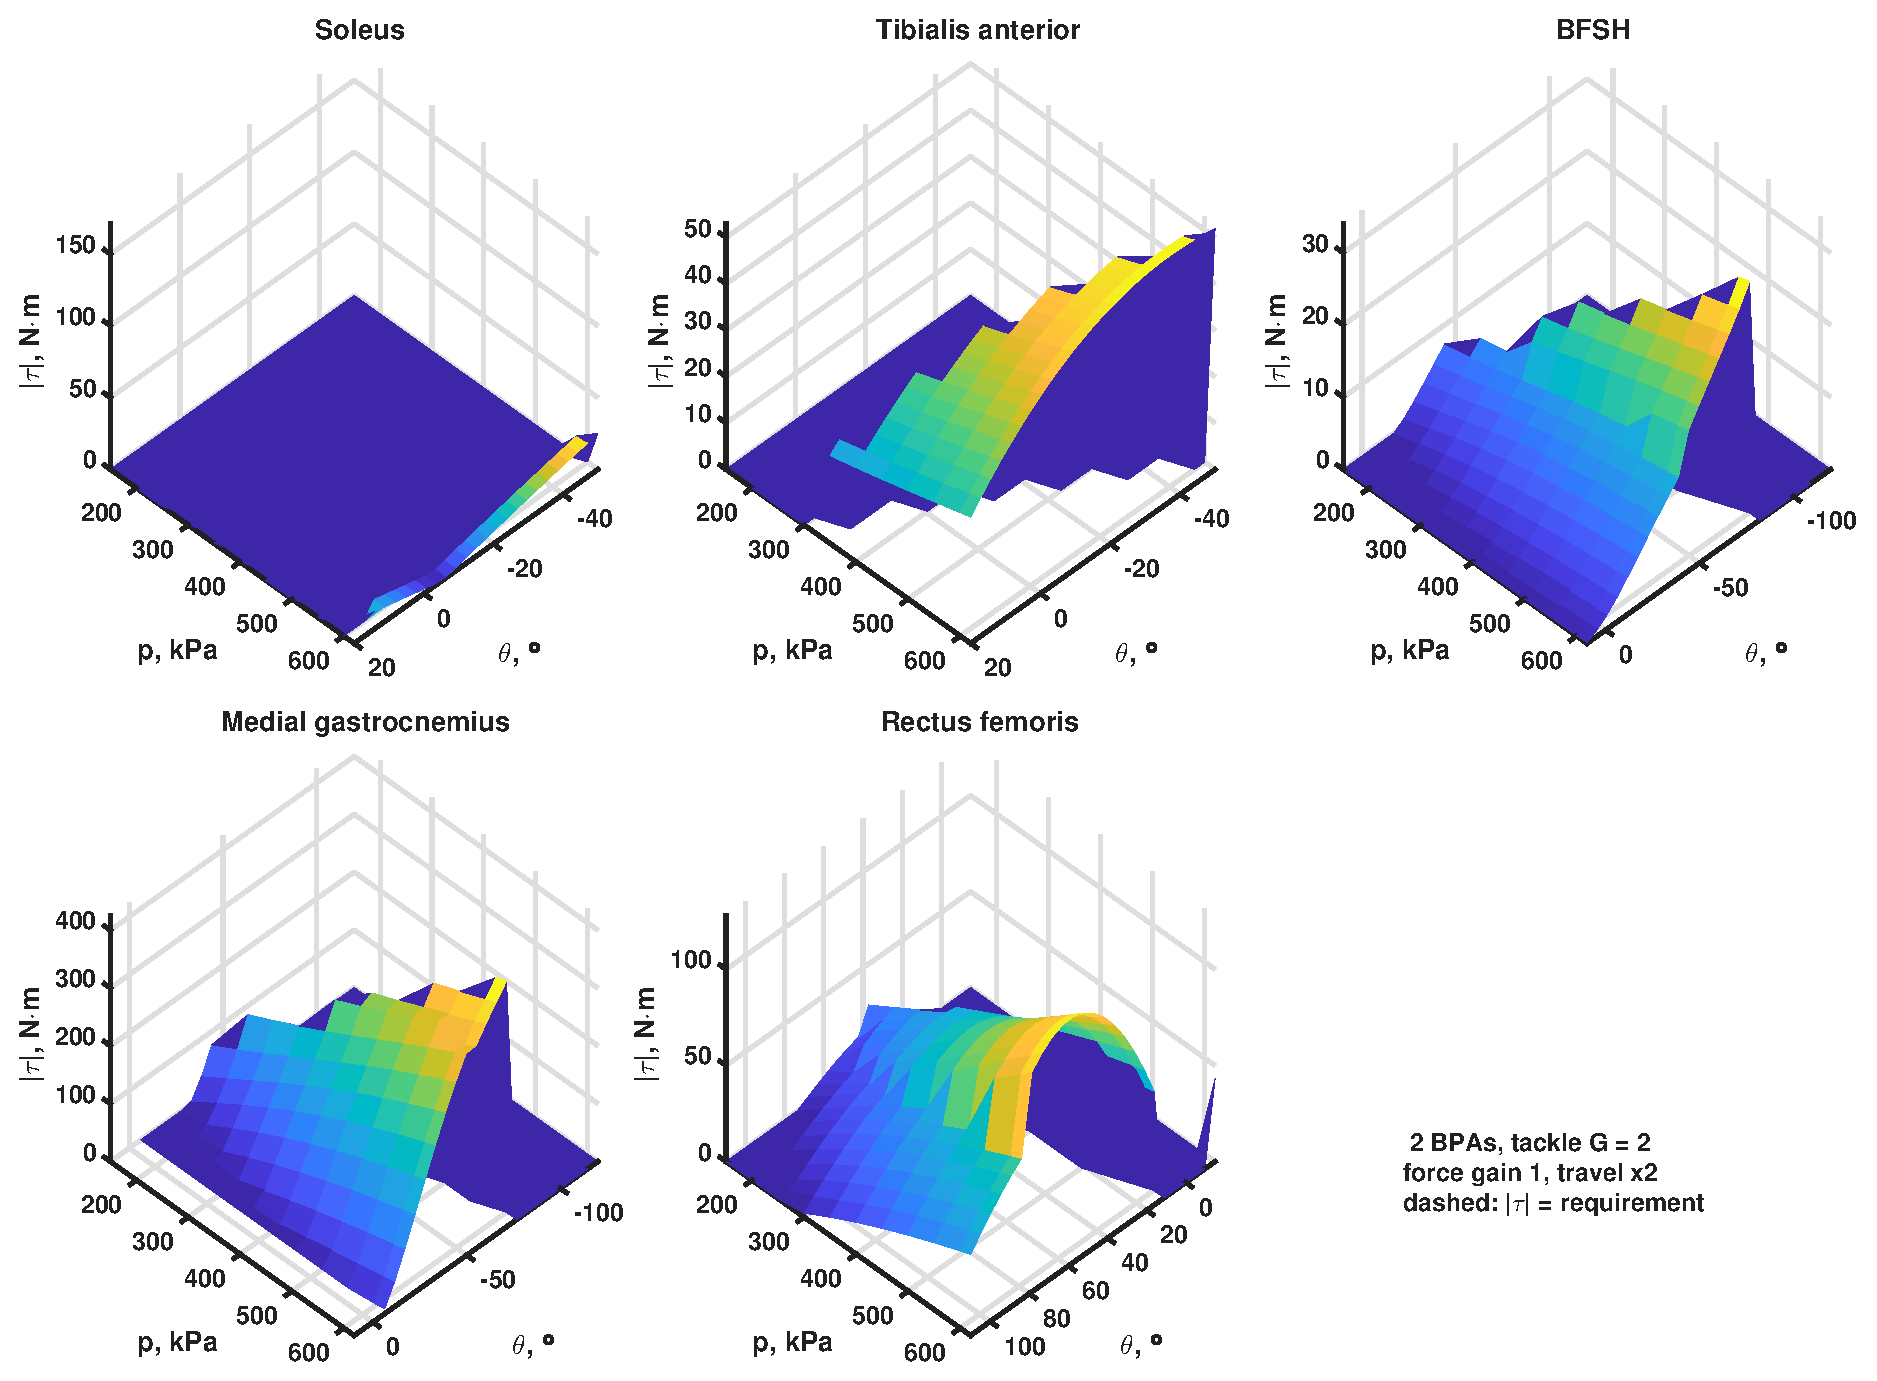
\includegraphics[width=1.0\textwidth]{Figures/PulleyTorqueSurfaces_20261020.eps}
\end{center}
\caption{Predicted insertion-torque magnitude over joint angle and supply pressure at the re-solved doctrine configuration of a parallel BPA pair through a two-part tackle (force gain 1, travel gain 2); the black dashed curve marks where the magnitude equals the human requirement, so the requirement is met above the curve. Panels show \textbf{(A)} soleus and \textbf{(B)} tibialis anterior over the ankle, \textbf{(C)} biceps femoris short head over the knee, \textbf{(D)} medial gastrocnemius over the knee with the ankle pinned at zero, and \textbf{(E)} rectus femoris over the hip of its recorded route; the soleus requirement lies above the plotted range, so it draws no curve. Joint angles are negative in flexion, and the tendon exit follows the moving-force-point routing throughout.}\label{fig:PulleyTorqueSurfaces}
\end{figure}

\begin{figure}[H]
\begin{center}
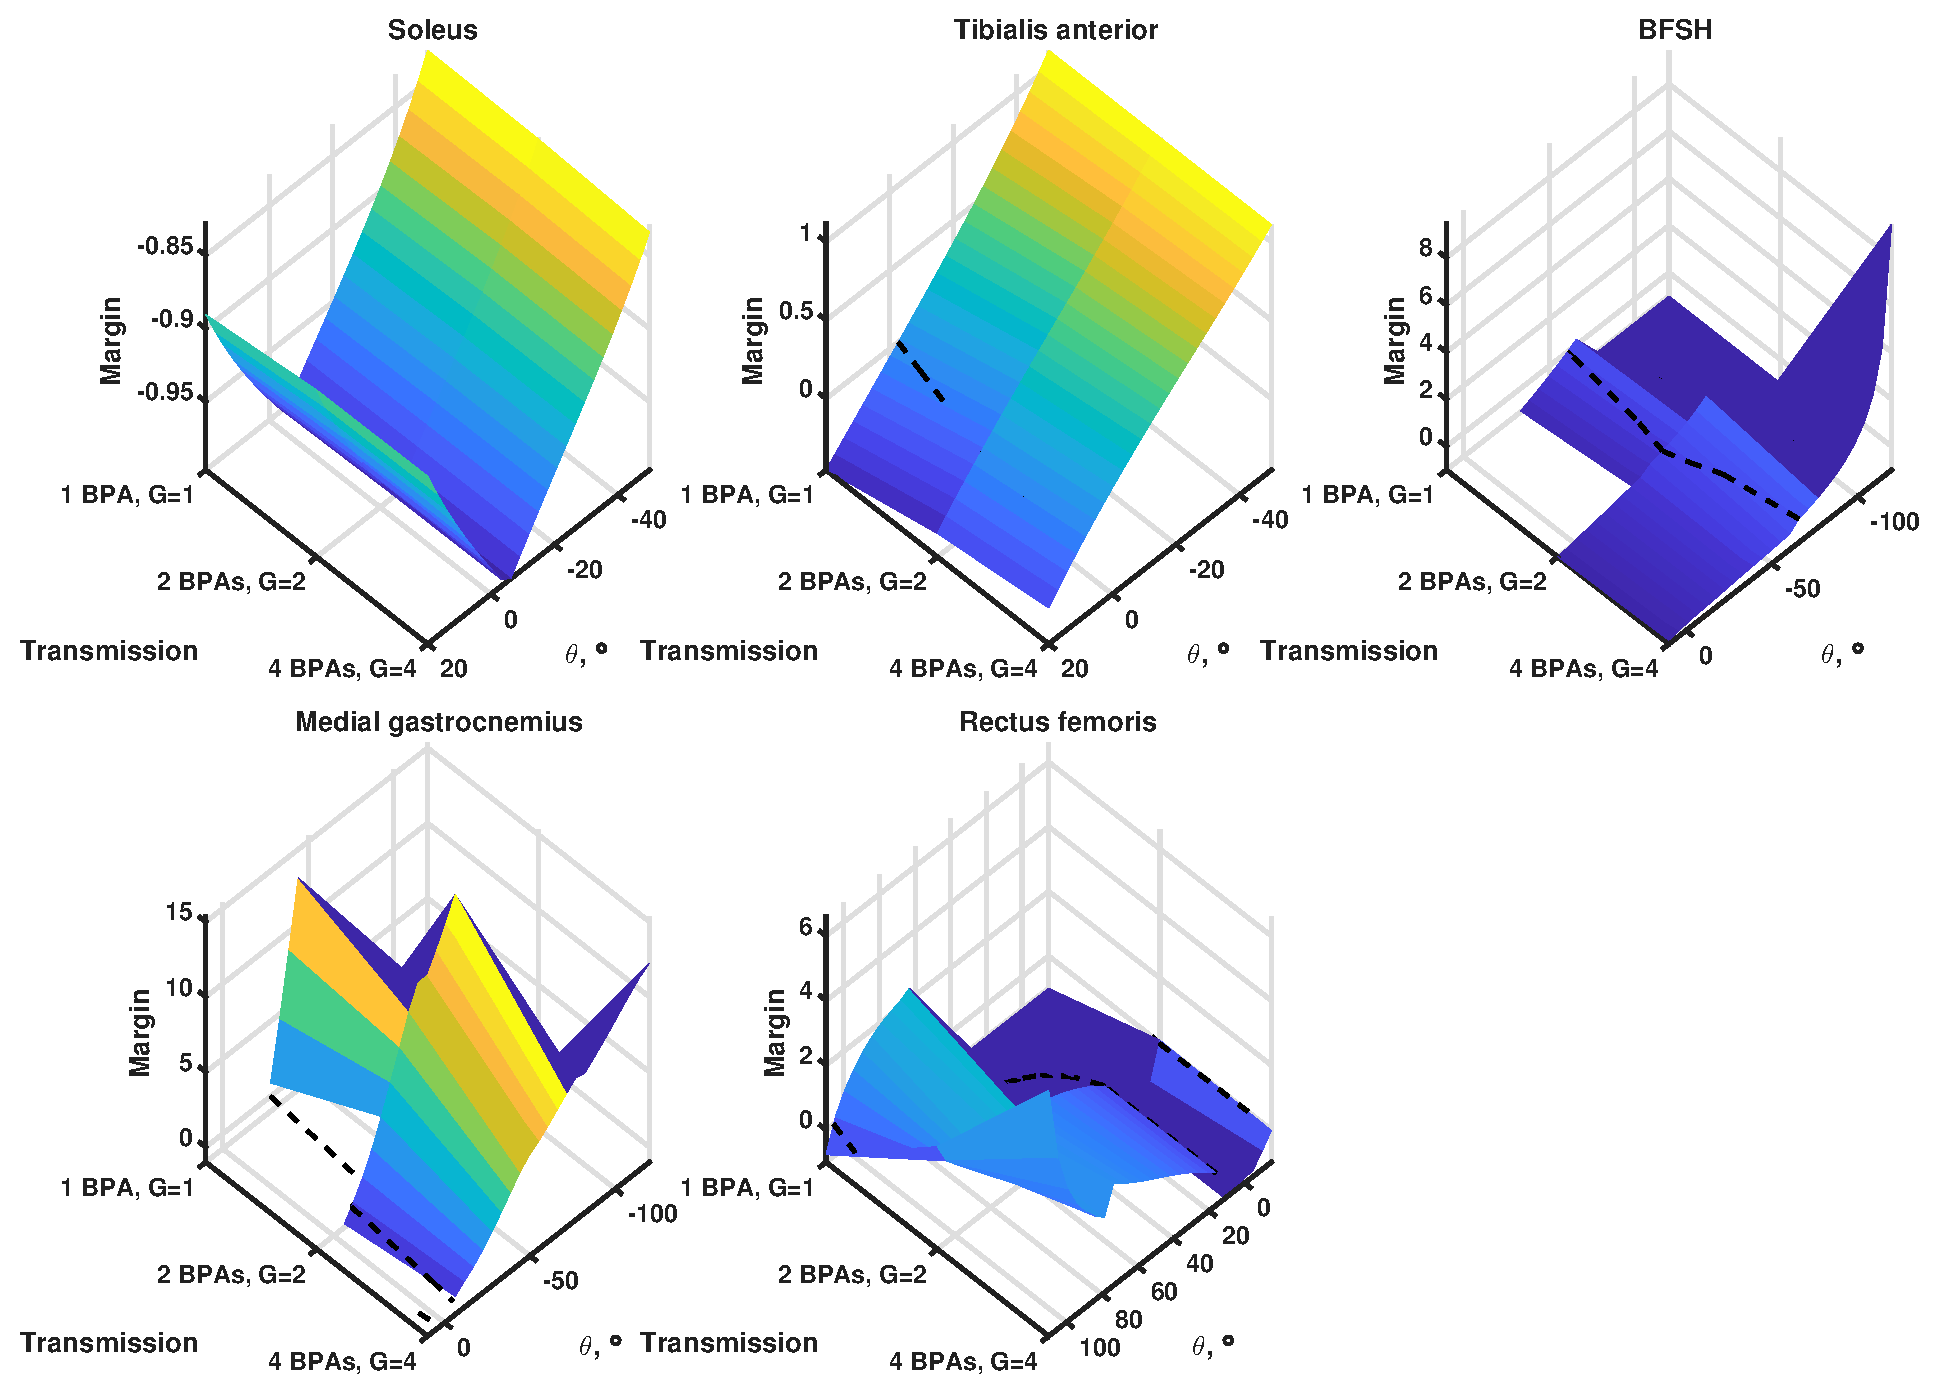
\includegraphics[width=1.0\textwidth]{Figures/PulleyMarginSurfaces_20261020.eps}
\end{center}
\caption{Torque margin over the human requirement versus joint angle at \qty{620}{\kPa} along the transmission ladder: the single-actuator baseline, a parallel BPA pair through a two-part tackle, and a four-actuator group through a four-part tackle, the latter two at matched net force; the margin is the fractional excess of the predicted torque magnitude over the required magnitude, the black dashed curve marks zero, and the requirement is met where the surface rises through it. Panels and evaluation planes follow Figure~\ref{fig:PulleyTorqueSurfaces}, and the biceps femoris short head is graded against the recorded requirement of its mono-pulley run.}\label{fig:PulleyMarginSurfaces}
\end{figure}

Physical validation of the redesigned extensor route has begun. In the first test of the $\diameter$\qty{20}{\mm} extensor on the rebuilt route, three isometric points were held near full extension: measured knee torque of \qty{1.163}{\newton\meter} at \ang{10}, \qty{7.849}{\newton\meter} at \ang{11}, and \qty{23.437}{\newton\meter} at \ang{10}, against hung loads of \qtylist{3.7;25.2;76}{\newton} at gauge pressures of \qtylist{388.5;388;592}{\kPa}. The first and third points sit at essentially the same knee angle and span a twentyfold range of held torque, so they begin to map the route's response near extension as pressure and load vary. The full angle sweep, and the corresponding flexor measurements, are pending.

The same pipeline was extended from the knee to all 27 muscle-actuators of the robot-body model, and we report that extension as a status rather than a completed result. The first pass reached 19 of the 27 actuators, and its chosen routes showed the penalty-based formulation to be the binding limitation: all but one violated the feasibility constraints, the exception being the biceps femoris long-head pair at a worst-angle margin of $+0.03$~\%, indistinguishable from zero. The formulation was then restructured so that the task envelope, the joint-angle window each route must serve, acts as a hard feasible set rather than a penalty. In the restructured pass, twelve actuators terminated when the route builder failed while assembling the redesigned path segments, an implementation failure of the optimization pipeline rather than a property of the routes, leaving fifteen finalized routes; eight were chosen from constraint-feasible configurations (semimembranosus, biceps femoris long head, tensor fasciae latae, soleus, lateral gastrocnemius, tibialis anterior, iliacus, and psoas), and six of those met the torque requirement at every angle, with worst-angle margins from $+0.25$~\% (biceps femoris long head) to $+250.7$~\% (tensor fasciae latae). All of these redesign solutions remain optimizer-stage results: the reference model contains no pulley entities, no via points or markers were added to it for these routes, and the redesigned geometry has not yet been propagated into the dynamic simulation models.

\subsection{Design Factors for Isometric Torque}\label{sec:design_factors}

Read as a design problem, isometric torque about a BPA-actuated joint factors into three quantities the designer controls: the moment arm $r$, the normalized contraction $\varepsilon^{*}$ at which the actuator operates, and the compliance of the path and its fixtures, carried by the $\chi$ terms. Each result in this paper maps onto one corner of that triangle. Short moment arms amplify every error, so stiffness must be budgeted where the arm is short \citep{young_analyzing_2019}. The route should keep $\varepsilon^{*}$ high through the functional range, because the wrapping loss of Equation~(\ref{eq:deltaL}) scales with $(1 - \varepsilon^{*})^{2}$ and therefore grows exactly where an under-contracted actuator is weakest. Moment arm and contraction budget trade against each other, and the cam redesign shows the trade can be favorable: it raises the moment arm from the direct route's \qty{44.9}{\mm} to \qty{61.2}{\mm} to a span of \qty{59.4}{\mm} to \qty{102.8}{\mm} while improving the torque margin. Pressure headroom, finally, is a design resource: the cam route meets its envelope between \qty{269}{\kPa} and \qty{507}{\kPa} against a \qty{620}{\kPa} ceiling.

These factors situate our work among musculoskeletal robot legs. Multifilament muscle routing has produced human-scale lower limbs \citep{kurumaya_musculoskeletal_2016}, anthropomorphic arms \citep{hitzmann_anthropomorphic_2018}, and full human-mimetic humanoids \citep{asano_musculoskeletal_2019}, and tendon-driven bodies have supported investigations from reflexive hopping \citep{liu_robotic_2018} to human-like manipulation \citep{chen_realizing_2019} and cognitive locomotion \citep{schilling_adaptive_2022}. Linkage-based knees manage the moment-arm problem geometrically \citep{romero_four-bar_2020}, reviews of dynamic multilegged robots treat actuation routing as a first-order design decision \citep{he_mechanism_2020}, and tunable-compliance actuators make fixture compliance a design element rather than an error source \citep{leibach_development_2020}. What these designs share with ours is the recognition that the attachment route, not the actuator alone, sets the deliverable torque. What the corrected model adds is a quantitative accounting of the compliance and wrapping losses along that route, so that a route can be designed against a torque target rather than checked after the fact. \citet{morrow_optimization_2020} optimized artificial-muscle placement on a bipedal robot with a rigid-body torque model, and the correction terms quantified here are the physics such rigid-body placements leave unmodeled.

The correction family also complements the BPA force-modeling literature. Static models of the actuator in isolation, from the classical McKibben analyses \citep{chou_measurement_1996} through approximation formulas \citep{sarosi_new_2012} to geometrically grounded models of the Festo muscle \citep{martens_modeling_2017, tondu_static_2022}, describe the actuator itself; none of them carries attachment compliance, length offsets, or wrapping losses into a joint-torque prediction. The terms validated here attach to the force characterization of \citet{bolen_2026} and travel with it across joint configurations under one consistent parameter set.

\subsection{Limitations and Future Work}\label{sec:limitations}

The redesign results carry caveats that bound their use. The flexor redesign solves its second actuator's endpoints from the first by the mirrored-endpoint rule rather than optimizing the two routes independently, so the mirror symmetry is built into the design; freeing the second route's endpoints is the next design refinement. All redesign solutions are optimizer-stage: they have not been propagated into the simulation models, and the physical validation rests on three torque points near full extension, with the full sweep and the flexor measurements pending. The stiffness pair itself was selected by an external design requirement rather than uniquely identified, because the pinned-flexor data admit a family of near-equivalent pairs; an independent stiffness measurement of the test stands would close that non-identifiability and either confirm or replace the adopted pair. The wrapping factor $\chi_{3}$ was identified on the $\diameter$\qty{10}{\mm} extensor family and applied unchanged to the $\diameter$\qty{20}{\mm} redesigns, so its transfer across actuator diameters is untested. On the characterization side, the fictive-strain formulation inherits the conclusion of our force characterization that the unloaded \qty{620}{\kPa} contraction $\varepsilon_{620}$ should be recorded for each actuator used on a robot \citep{bolen_2026}, since every correction term is normalized by it. The whole-body extension identified its own next steps: the route-builder assembly failure needs a fix before the twelve terminated routes can be rebuilt, and the two torque-short feasible routes need either larger actuators or relaxed corridors. One scope statement, finally, belongs with these caveats: the correction terms are identified for these test stands and this actuator family, and other joints or actuator sizes should repeat the two-stage procedure rather than reuse the values. That procedure is inexpensive next to the test campaign it saves, which is the point of having it.

\section{Conclusion}\label{sec:conclusion}

This work asked what a braided pneumatic actuator actually delivers about a joint, and answered with a corrected torque model and the design workflow built on it. Isometric knee-torque measurements on pinned and biomimetic test stands, interpreted through a hybrid calculation that substitutes the measured muscle length and moment arm, isolated the error sources that rigid-body torque models miss: attachment compliance, a constant effective-length offset, and a wrapping loss that acts like fictive strain, expressed through the unloaded \qty{620}{\kPa} contraction of the free actuator. A two-stage identification recovered the correction terms with one stiffness pair shared across the flexor and extensor configurations, roughly halving fitting-set error, cutting held-out error by two thirds or more, and carrying the corrected model from the pinned knee to the biomimetic knee without refitting. The attachment routes themselves were then redesigned under the corrected model: two $\diameter$\qty{20}{\mm} actuators per route, graded against OpenSim human isometric torque profiles with a required \qty{5}{\percent} overshoot, meet or exceed the human flexor and extensor envelopes at every angle, the cam extensor design converts the thinnest margins into design headroom, the pulley surfaces quantify how a reeved tackle, fed by parallel actuator pairs, converts surplus force into range of motion across five muscle sites, and the first physical torque points of the redesigned extensor route have been measured near full extension. The design-factor reading is the practical summary: moment arm, normalized contraction, and path compliance are the three quantities a designer of BPA-actuated joints controls, and each now carries a measurable, correctable model. First-iteration torque design for such joints is, as a result, no longer a guess.

\section*{Resource Identification Initiative}
\begin{itemize}
    \item MATLAB (RRID:SCR\_001622)
    \item OpenSim (RRID:SCR\_002683)
    \item Arduino UNO (RRID:SCR\_017284)
\end{itemize}

%To take part in the Resource Identification Initiative, please use the corresponding catalog number and RRID in your current manuscript. For more information about the project and for steps on how to search for an RRID, please click \href{http://www.frontiersin.org/files/pdf/letter_to_author.pdf}{here}.


\section*{Conflict of Interest Statement}
The authors declare no conflicts of interest. The funders had no role in the design of the study; in the collection, analysis, or interpretation of data; in the writing of the manuscript; or in the decision to publish the results.

\section*{Author Contributions}
Conceptualization, B.B. and C.M.; Methodology, B.B., C.M., and A.H.; Software, B.B., C.M., and L.B.; Validation, B.B. and A.H.; Formal Analysis, B.B.; Investigation, B.B., C.M., and L.B.; Resources, B.B., L.B., and A.H.; Data Curation, B.B.; Writing – Original Draft Preparation, B.B.; Writing – Review \& Editing, B.B., C.M., L.B., and A.H.; Visualization, B.B. and A.H.; Supervision, B.B. and A.H.; Project Administration, B.B. and A.H.; Funding Acquisition, A.H.

\section*{Funding}
Research for this article was funded by the Department of Mechanical and Materials Engineering at Portland State University, the National Science Foundation (NSF) grant for NeuroNex: Communication, Coordination, and Control in Systems (C3NS) 2015317 and NSF grant 1943483. 

%Details of all funding sources should be provided, including grant numbers if applicable. Please ensure to add all necessary funding information, as after publication this is no longer possible.

\section*{Acknowledgments}
The authors would like to acknowledge the contribution of Alex Steele, who designed the initial biomimetic 4-bar knee linkage we used for the test. He gave us solid models, built a 3D prototype, and let us break said prototype. His prompt and thoughtful responses to our questions about the previous design was very much appreciated. The authors would also like to thank Jasmine Bradley for her help reworking the figures in the results section. As a visual designer, her contributions improved the aesthetic quality and accessibility of the images. 
%This is a short text to acknowledge the contributions of specific colleagues, institutions, or agencies that aided the efforts of the authors.

\section*{Supplemental Data}
Supplemental Data includes figures for the test setup. 
 
 %\href{http://home.frontiersin.org/about/author-guidelines#SupplementaryMaterial}{Supplementary Material} should be uploaded separately on submission, if there are Supplementary Figures, please include the caption in the same file as the figure. LaTeX Supplementary Material templates can be found in the Frontiers LaTeX folder.

\section*{Data Availability Statement}
The data sets are available from the authors upon reasonable request.

%The datasets [GENERATED/ANALYZED] for this study can be found in the [NAME OF REPOSITORY] [LINK].

% Please see the availability of data guidelines for more information, at https://www.frontiersin.org/about/author-guidelines#AvailabilityofData

\bibliographystyle{Frontiers-Harvard} %  Many Frontiers journals use the Harvard referencing system (Author-Date), to find the style and resources by journal: https://zendesk.frontiersin.org/hc/en-us/articles/360017860337-Frontiers-Reference-Styles-by-Journal. For Humanities and Social Sciences articles please include page numbers in the in-text citations 
%\bibliographystyle{Frontiers-Vancouver} % Many Frontiers journals use the numbered referencing system (Author-date), to find the style and resources by journal: https://zendesk.frontiersin.org/hc/en-us/articles/360017860337-Frontiers-Reference-Styles-by-Journal
\bibliography{BolenFrontiers22}

%%% Make sure to upload the bib file along with the tex file and PDF
%%% Please see the test.bib file for some examples of references

\clearpage
\section*{Figures}

%%% Please be aware that for original research articles we only permit a combined number of 15 figures and tables, one figure with multiple subfigures will count as only one figure.
%%% Use this if adding the figures directly in the mansucript, if so, please remember to also upload the files when submitting your article
%%% There is no need of adding the file termination, as long as you indicate where the file is saved. In the examples below the files (logo1.eps and logos.eps) are in the Frontiers LaTeX folder
%%% If using *.tif files convert them to .jpg or .png
%%%  NB logo1.eps is required in the path in order to correctly compile front page header %%%

%Frontiers requires figures to be submitted individually, in the same order as they are referred to in the manuscript. Figures will then be automatically embedded at the bottom of the submitted manuscript. Kindly ensure that each table and figure is mentioned in the text and in numerical order. Figures must be of sufficient resolution for publication \href{https://www.frontiersin.org/about/author-guidelines#ImageSizeRequirements}{see here for examples and minimum requirements}. Figures which are not according to the guidelines will cause substantial delay during the production process. Please see \href{https://www.frontiersin.org/about/author-guidelines#FigureRequirementsStyleGuidelines}{here} for full figure guidelines. Cite figures with subfigures as figure \ref{fig:2}B.

%%% If you are submitting a figure with subfigures please combine these into one image file with part labels integrated.
%%% If you don't add the figures in the LaTeX files, please upload them when submitting.
%%% Frontiers will add the figures at the end of the provisional pdf automatically
%%% The use of LaTeX coding to draw Diagrams/Figures/Structures should be avoided. They should be external callouts including graphics.

\section*{Tables}

%Tables should be inserted at the end of the manuscript. Please build your table directly in LaTeX.Tables provided as jpeg/tiff files will not be accepted. Please note that very large tables (covering several pages) cannot be included in the final PDF for reasons of space. These tables will be published as \href{http://www.frontiersin.org/about/author-guidelines#SupplementaryMaterial}{Supplementary Material} on the online article page at the time of acceptance. The author will be notified during the typesetting of the final article if this is the case. 


\end{document}
